\documentclass{DeustoFDP}
\usepackage{hologo} % Paquete no necesario. Borrar en la memoria final al sustituir el texto
\hypersetup{
pdfauthor={Aitor Brazaola Vicario},
pdftitle={Proyecto de fin de grado de Aitor Brazaola en la Facultad de Ingeniería de la Universidad de Deusto},
}

\bibliography{bib}

\begin{document}

\frontmatter
\pagestyle{plain}

% Las siguientes lineas (21--26) se pueden eliminar del documento final.
% Notese que en ese caso es necesario descomentar la linea 28 para que las
% paginas esten correctamente numeradas.
\begin{titlepage}
    \newgeometry{left=0cm,right=0cm,bottom=0cm,top=0cm}
    
\includegraphics{fig/portada}
    \restoregeometry
\end{titlepage}
\cleardoublepage

\setcounter{page}{3}

\chapter*{Resumen}
El estilo de vida de la sociedad actual se aleja mas del contacto entre vecinos
que siempre ha existido en todas las comunidades en el que se propicia el
intercambio de bienes, favores y en muchos casos información vital para todos
los habitantes de la comunidad. Además, el crecimiento de las ciudades hace
que conocer las necesidades y preocupaciones de los habitantes cada vez sea una
tarea más difícil para los ayuntamientos.

Auzonet, como plataforma digital centrada en la comunidad de vecinos proporciona
el marco perfecto para que por un lado los vecinos dispongan una plataforma web
donde intercambiar toda esta información y por otro una fuente de datos para
ayuntamientos y terceras empresas.

\vspace{2em}

{\Large\bfseries\sectionfont Descriptores}
\vspace{3\medskipamount}

OpenData, Web, App, Red social.

\cleardoublepage\tableofcontents
\cleardoublepage\listoffigures
\cleardoublepage\listoftables
\cleardoublepage\listoflistings

\mainmatter
\pagestyle{phdthesis}

\chapter{Introducción}\label{cha:introduccion}
El objetivo de este proyecto es el de crear una plataforma social online de la que se vean beneficiadas diferentes partes, por un lado, los propios vecinos como nexo de unión de la comunidad de forma que se disponga de un lugar accesible a través de internet donde se puedan publicar avisos o información de forma permanente correspondientes a la comunidad en una corchera virtual, símil de la física que existe habitualmente en los portales, y poder publicar peticiones u ofrecimientos de objetos o servicios permitiendo la interacción de los interesados a través de la plataforma.

Por otro lado, la información generada por el uso de la plataforma puede suponer una fuente de datos de gran calidad para los servicios de los ayuntamientos, de forma que gracias al análisis de los mismos se pueden tomar decisiones en función de las necesidades reales que predominen más en cada barrio.

Este proyecto se tiene que desarrollar sobre la base del proyecto Europeo WeLive ~\cite{WeLive} del que DeustoTech~\cite{DeustoTech} Morelab ~\cite{Morelab} forma parte, utilizando las librerías e interfaces de programación que pone a disposición. WeLive es una plataforma web para la promoción del OpenData creada por diversas entidades europeas que proporciona una serie de servicios para desarrolladores y para entidades públicas con el fin de la difusión de los datos y la explotación de los mismos en aplicaciones de terceros sin coste alguno.

Los principales retos a los que va a hacer frente este proyecto son:

\begin{itemize}
    \item La creación de un portal web social con las funciones requeridas.
    \item La explotación de datasets públicos que aporten valor a la aplicación.
    \item La creación de nuevos datasets en función del uso.
    \item La creación de una aplicación móvil capaz de interactuar con su símil en la web mediante una interfaz.
    \item La creación de un portal de análisis de datos que muestre la información de forma visual y significativa.
\end{itemize}

Además, durante el desarrollo puede que se necesiten desarrollar nuevos componentes de software que permitan personalizar la integración con WeLive y que puedan ser reulitizados en otros proyectos futuros poniéndolos a disposición pública en el repositorio de aplicaciones de WeLive.

Este proyecto va a necesitar capacidad técnica y habilidades interpersonales para lograr una buena colaboración entre los equipos de WeLive y de Auzonet para lograr crear la mejor solución posible.

Para llevar a cabo de desarrollo principal de la aplicación, se va a utilizar un framework de desarrollo web que permita implementar la mayor parte de las funciones de la aplicación web con la mínima reutilización de código y la mayor eficiencia, al igual que cuando se desarrolle la aplicación móvil, se va a necesitar emplear un framework que permita desarrollar al mismo tiempo para todos los sistemas operativos que existen actualmente en el mercado.

Las herramientas previamente citadas añaden el reto de la realización de una investigación acerca de la actualidad de los frameworks de desarrollo web y móvil valorando las ventajas y desventajas con respecto al proyecto y el aprendizaje del modelo de comunicación que requiere WeLive para interactuar con los datos públicos.

Todas las fases del desarrollo van a demostrar de forma exhaustiva los conocimientos adquiridos durante la universidad y además requerirán del aprendizaje de conocimientos nuevos, tanto técnicos como teóricos.

En este documento se describirá el proyecto y se hará una aproximación a las soluciones más parecidas que existen a día de hoy y se hablará de la importancia del Open Data y lo que aporta a la sociedad, se describirá el proyecto WeLive y todas las posibilidades que ofrece.

Después se describirá la planificación, así como las fechas de desarrollo y las diferentes tareas y las cargas de trabajo y el diagrama de Gantt.

A continuación se pasará a describir el propio desarrollo de Auzonet, razonando las herramientas que finalmente se han empleado y los motivos de su elección, así como la propia estructura del proyecto y las posibles divisiones funcionales de los componentes del software, su diseño y requerimientos.


Para terminar, se presentarán las conclusiones halladas a lo largo de todo el proceso de creación y se tomará información acerca de el uso en las pruebas programadas para futuros proyectos.

\section{Antecedentes y justificación}\label{cha:antecedentesyjustificacion}
La creación de una red social de vecinos en la que todos los miembros de cada portal o comunidad puedan interactuar entre ellos compartiendo recursos e información no es una iniciativa nueva, en otros países como Alemania o Estados Unidos se han creado proyectos similares \cite{larazon}, internet ha supuesto un antes y un después en la creación de comunidades de todo tipo de ámbitos, sin embargo, no se encuentran propuestas que se beneficien del creciente auge de la publicación por parte de las entidades públicas datos, que en muchos casos, son la fuente más fiable sobre la que construir aplicaciones y servicios para los propios ciudadanos.

Si bien es cierto que actualmente, muchas entidades públicas ponen a disposición estos datos de forma digital por la imagen de transparencia que provoca, no son conscientes de la utilidad real de los mismos, es por eso que durante el desarrollo de este proyecto, se han dado casos, en los que los datos se han encontrado mal formateados y ha habido que solicitar modificaciones a los organismos involucrados.

El hecho de que la mayor parte de datasets que son publicados por organizaciones públicas no son empleados en sistemas creados por terceros, provoca cierta despreocupación en el estado e integridad de los mismos.

Este proyecto trata de unir las capacidades de comunicación entre personas que brinda la red con los beneficios que aporta el Open Data a los ciudadanos, algo que como se ha comprobado no se ha podido encontrar iniciativas similares.

\chapter{Objetivos y alcance}\label{cha:objetivosyalcance}
\section{Resumen del proyecto}
El estilo de vida de la sociedad actual en constante cambio ha hecho que se pierda en mayor medida la interacción y la relación entre vecinos que ha existido tradicionalmente en los portales de las viviendas donde antes era común la colaboración para muchos aspectos de la vida cotidiana, encontrar a una persona capaz de sintonizar los canales de la televisión o que pueda cuidar de los niños un día que el trabajo lo impida por citar un par de ejemplos.

Para solventar esta problemática se ha pensado en aprovechar las ventajas que ofrece la tecnología y en concreto internet creando una plataforma social donde poder replicar la experiencia anteriormente descrita desde un teléfono inteligente o un portal web accesible desde cualquier ordenador conectado a internet.

\section{Definición del proyecto}
Auzonet debe cumplir las expectativas de al menos dos tipos de usuarios:
\begin{description}
    \item[Ciudadano:] Es el principal usuario del sistema, es el beneficiado de las funciones que ofrece la plataforma y el origen de la información que crea el sistema para explotación posterior.
    \item[Organización pública:] Es el que analiza los datos que genera la plataforma para elaborar estadísticas y promover servicios que mejoren la calidad de vida en las ciudades y de las personas.
\end{description}

Para lograr esto se va a desarrollar:
\begin{itemize}
    \item Una aplicación web donde los usuarios puedan registrar su comunidad de vecinos en función de los datos ya existentes publicados por el ayuntamiento de su ciudad, para que el resto de vecinos interesados puedan unirse a ella y beneficiarse de sus funciones.
    \item Una aplicación móvil que permita interactuar con las principales funciones de la web desde un teléfono inteligente.
\end{itemize}

\subsection{Funcionalidades}
Los usuarios tienen que poder buscar su portal entre los que muestra el formulario de registro de comunidad y agregar la información adicional requerida para poder registrarla en el sistema y comenzar a operar, en ese momento, el vecino responsable de crear la comunidad virtual tiene la opción de notificar vía email a quien desee mandar una solicitud de unión.

Cada usuario puede pertenecer a más de una comunidad de vecinos, teniendo en cuenta que puede querer estar al tanto de la comunidad de su domicilio habitual y por ejemplo el de las vacaciones.

Cada comunidad de vecinos representada en la aplicación tiene su propia página principal donde se puede ver la corchera con los avisos o notas informativas publicadas y una tabla inferior dividida en dos secciones llamadas Peticiones y Ofertas donde se visualizarán las disponibles en ese momento creadas por los miembros de esa comunidad.

Desde la página de inicio de cada comunidad, el usuario puede crear una petición de un producto o servicio o publicar una oferta en la que puede especificar si quiere que sea remunerada o gratis.

Para garantizar cierta confianza a la hora de colaborar con otro usuario, se creará un sistema de karma representado por un valor numérico que será mayor o menor mediante la votación de otros usuarios al terminar un acuerdo ya sea de oferta o de petición.

\subsection{Limitaciones}
Auzonet en ningún caso va a gestionar los pagos entre particulares, más allá del simple hecho de un historial de interacciones entre peticiones y ofrecimientos entre vecinos. Las partes interesadas en una transacción deberán acordar qué métodos utilizan para pagarse en caso de que lo requieran y es responsabilidad completa por su parte asegurarse de realizar la transacción en un marco económico legal.

Serán los propios usuarios los que en caso de querer utilizar la plataforma tendrán que buscar su portal en la sección destinada a la creación de comunidades y añadir los datos que la aplicación considere necesarios para poder hacer uso de las funciones del software.

No está previsto desarrollar aplicaciones con el kit de desarrollo nativo de cada sistema operativo móvil para evitar tener que mantener varios procesos de desarrollo simultáneos durante la creación de la aplicación móvil, se utilizarán tecnologías web que permitan desplegar la aplicación en los disponibles actualmente en el mercado, además, no se contempla que la aplicación móvil disponga de todas las funcionalidades de la aplicación web, se hará un estudio para decidir qué funcionalidades tienen mas sentido disponer de ellas en movilidad para primar la usabilidad por encima de la cantidad de opciones.

\chapter{Producto final}
El producto principal de este proyecto es la aplicación web con la que los usuarios van a interactuar en sus navegadores, acordar entre ellos ofertas y publicar información y avisos relativos a la comunidad a la que pertenecen, pudiendo incluso pertenecer a mas de una al contemplar casos de personas que tengan varias viviendas en propiedad. Adicionalmente, la aplicación móvil es el segundo producto que este proyecto quiere producir, añadiendo la posibilidad de gestionar todas las funciones de la web desde un dispositivo móvil.

Finalmente, se contempla la creación de un manual de usuario que detalle todas las funciones de la plataforma y un plan de pruebas en el que se pueda recoger retroalimentación.

\chapter{Descripción de la realización}
La realización de Auzonet se va a separar en unidades funcionales, en primer lugar se centrará en finalizar la aplicación web y después la móvil.

Como se puede ver en el EDT \ref{fig:edt} las fases del proyecto van a ser las siguientes:
\begin{description}
    \item[Requisitos:] Análisis de los principales requisitos funcionales.
    \item[Diseño:] Diseño de las estructuras de datos y lógicas que harán funcionar la aplicación, creación de maquetas y aproximación al diseño estético de la solución.
    \item[Desarrollo de la aplicación web:] Proceso de implementación de la aplicación principal, con la integración de WeLive y una interfaz con diseño "responsivo" que ayude a ser mostrado en dispositivos móviles.
    \item[Desarrollo de la aplicación móvil:] Proceso de implementación de la aplicación móvil que aprovechará el diseño "responsivo" de la web para mostrarse en pantallas de reducidas proporciones correctamente.
    \item[Pruebas:] Diferentes ejecuciones en distintos entornos de prueba para extraer la mayor cantidad de posibles fallos a depurar, se intentará involucrar a colaboradores y amigos del programador para que simulen un uso real de la plataforma y ayuden a detectar errores.
\end{description}

\section{Método de desarrollo}
Al tratarse de un proyecto en el que solo interviene un desarrollador, no van a ser empleadas metodologías ágiles que facilitan la cooperación y el trabajo en grupo, en su lugar, se empleará un sistema de listas de tickets con diferentes clasificaciones utilizando un software de gestión de tareas.

Las tareas se clasificarán de la siguiente forma:
\begin{table}[H]
   	\centering
   	\caption{Categorías de tickets.}\label{tab:presupuestoperfiles}
   	\begin{tabular}{cccc}
   		\toprule
   		\textbf{Categoría} & \emph{Descripción}\\
   		\midrule
   		Funcional  & Funciones que representan el núcleo de la aplicación.\\
   		No funcional   & Funciones que complementan y mejoran la experiencia de usuario.\\
   		Bug & Fallos pendientes de solucionar.\\
   		Mejora & Funciones que añaden utilidad a la plataforma.\\
   		\bottomrule
   	\end{tabular}
\end{table}

En ocasiones, determinadas tareas pueden venir de fuentes externas como sugerencias de mejora o fallos importantes detectados en una prueba, en ese caso, se añaden a la lista con la etiqueta correspondiente y se priorizan en función de su importancia.

\subsection{Productos intermedios}
\begin{itemize}
   	\item Aplicación web funcional.
   	\item Integración de los datos públicos de Bilbao con la plataforma WeLive.
   	\item Aplicación móvil funcional.
\end{itemize}
\newpage
\begin{figure}[H]
   	\centering
   	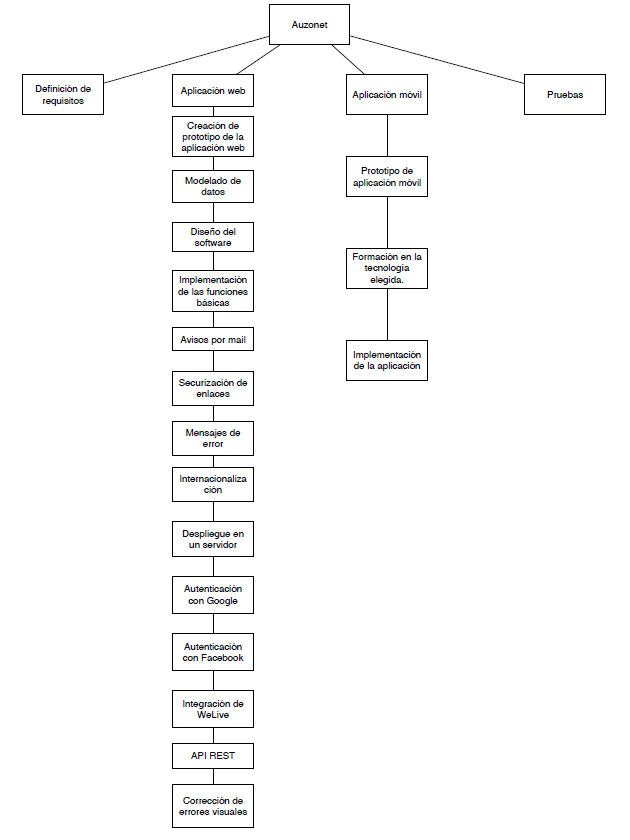
\includegraphics{fig/EDT}
   	\caption{EDT}\label{fig:edt}
\end{figure}

\newpage
\section{Tareas principales}
\begin{figure}[H]
	\centering
	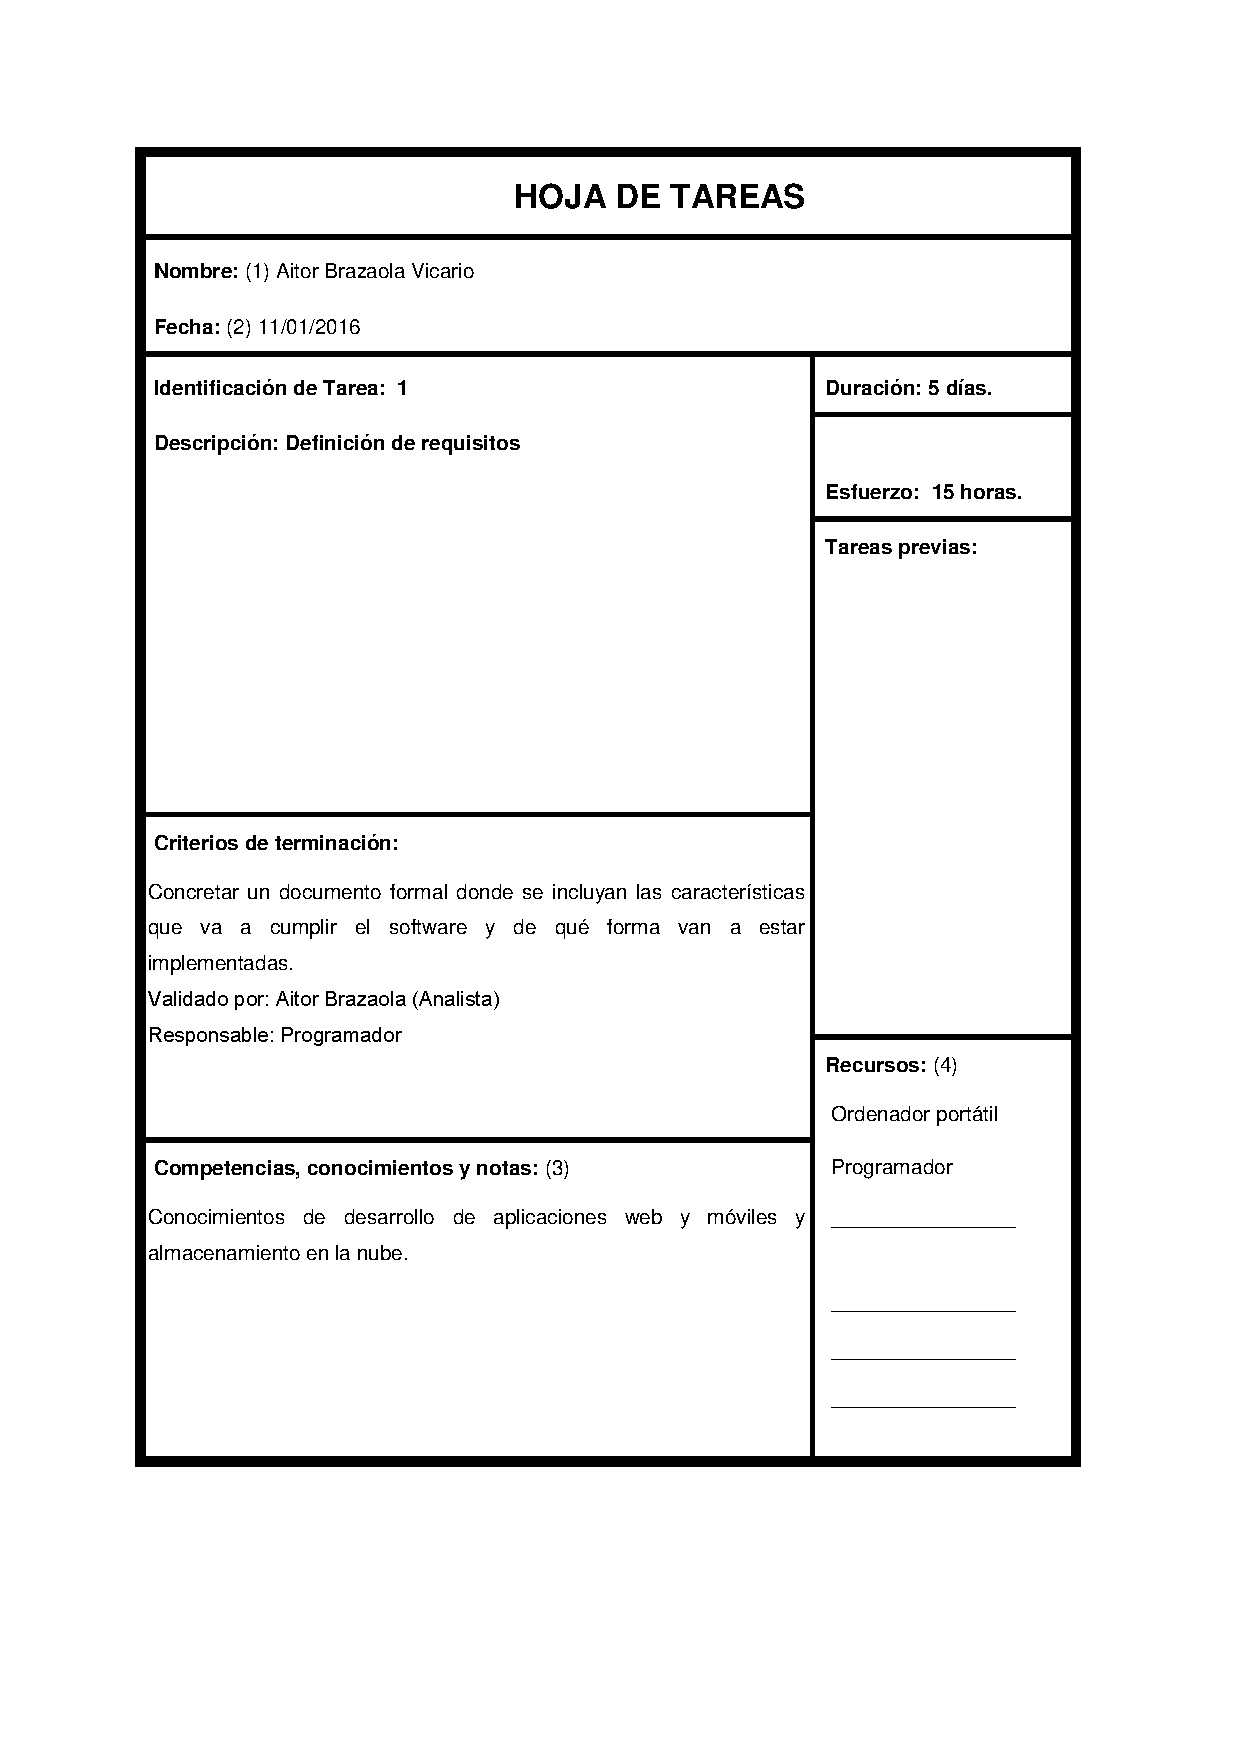
\includegraphics[width=0.9\textwidth]{fig/Tareas/1}
	\caption{Tarea 1}
	\label{fig:t1}
\end{figure}

\begin{figure}[H]
	\centering
	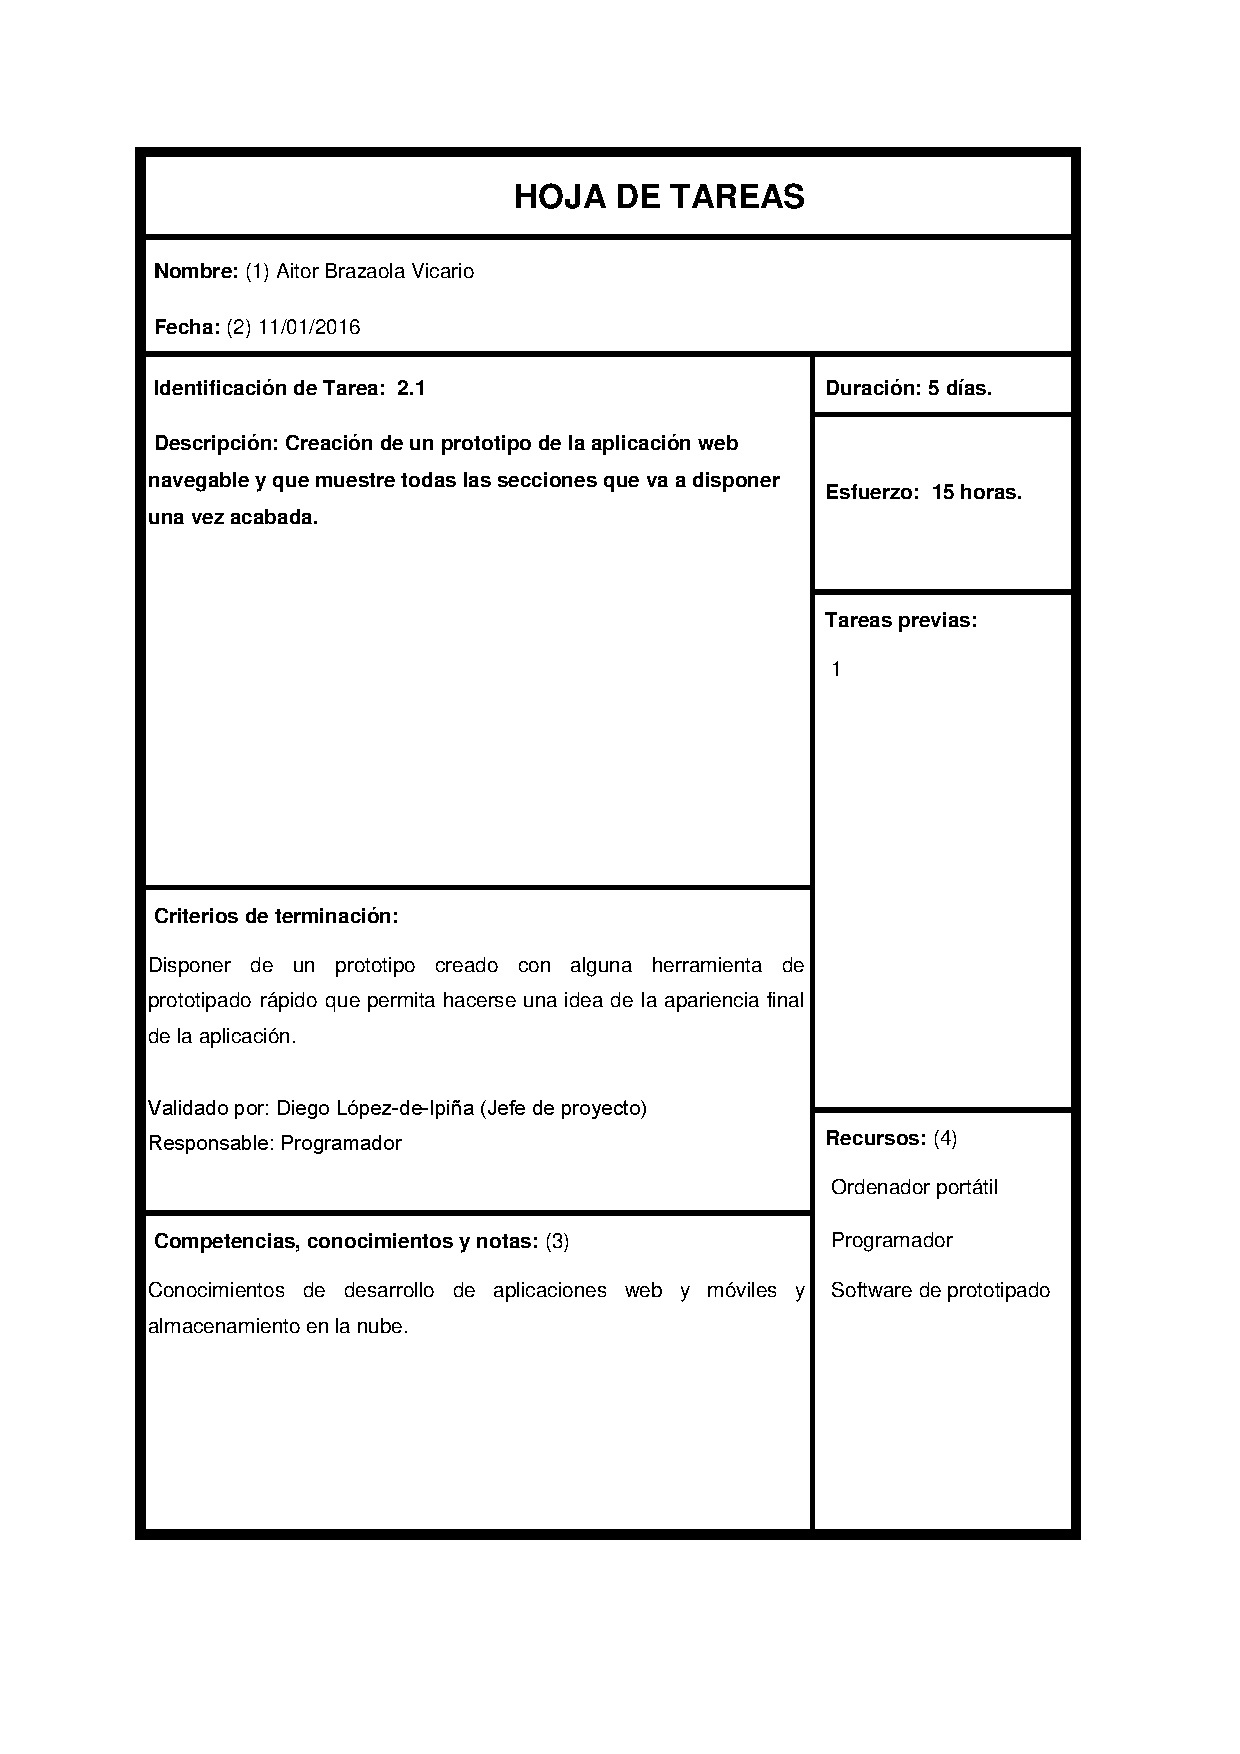
\includegraphics[width=0.9\textwidth]{fig/Tareas/21}
	\caption{Tarea 2.1.}
	\label{fig:t21}
\end{figure}

\begin{figure}[H]
	\centering
	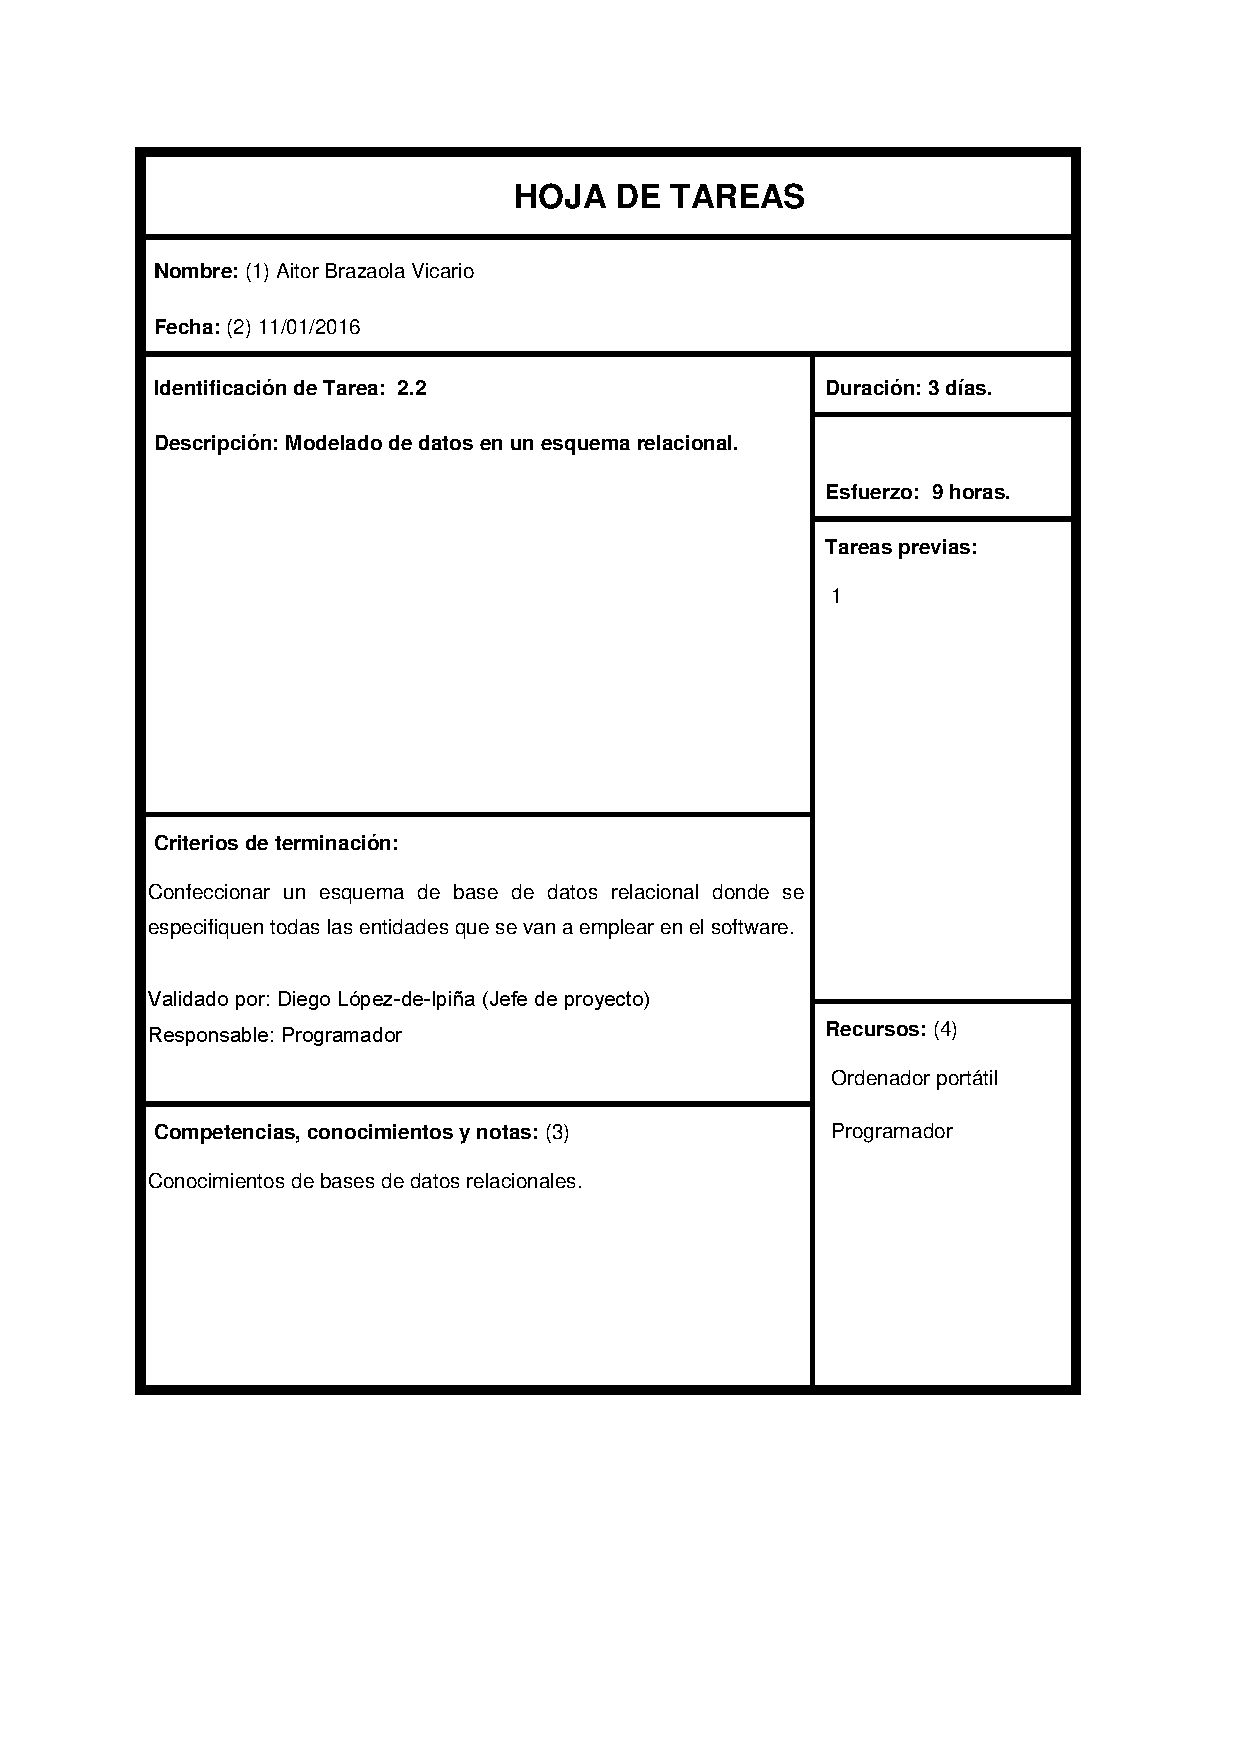
\includegraphics[width=0.9\textwidth]{fig/Tareas/22}
	\caption{Tarea 2.2.}
	\label{fig:t22}
\end{figure}

\begin{figure}[H]
	\centering
	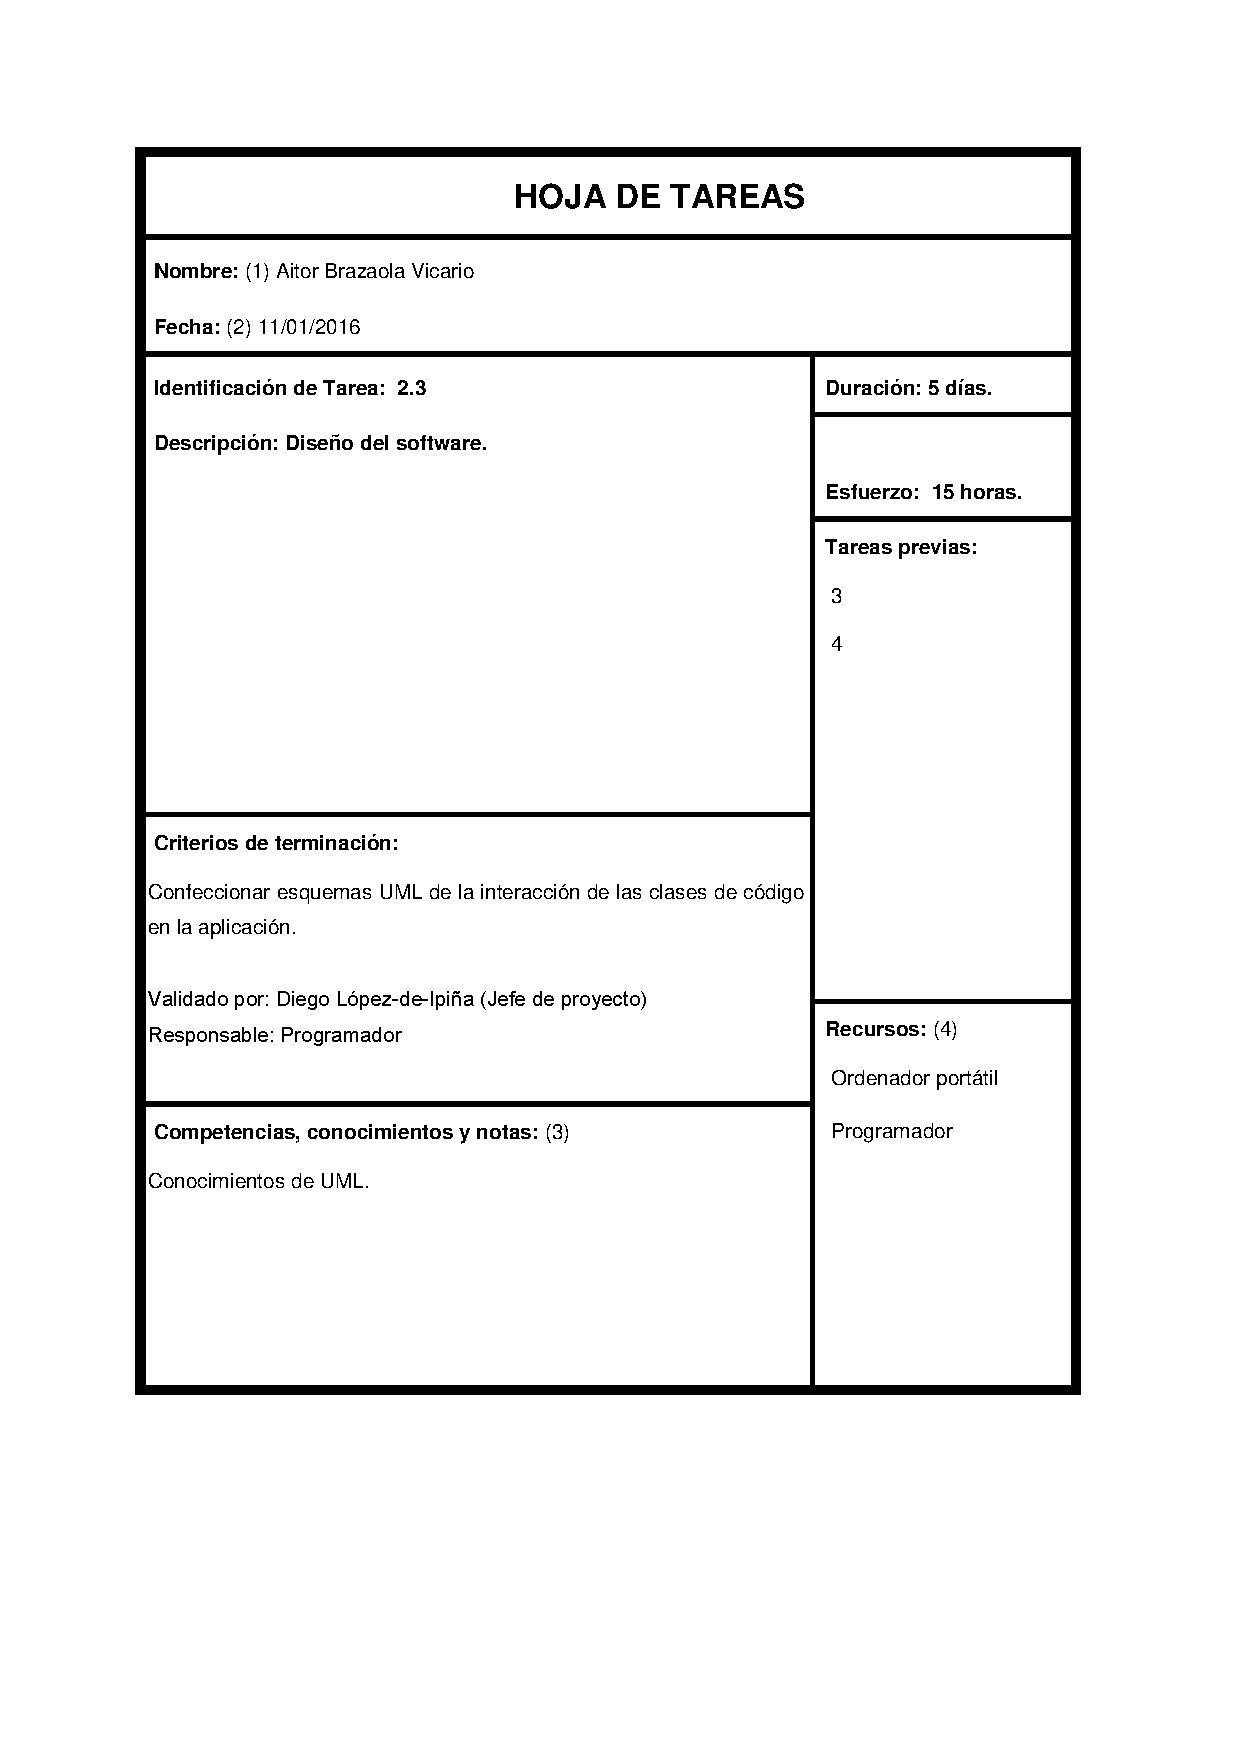
\includegraphics[width=0.9\textwidth]{fig/Tareas/23}
	\caption{Tarea 2.3.}
	\label{fig:t23}
\end{figure}

\begin{figure}[H]
	\centering
	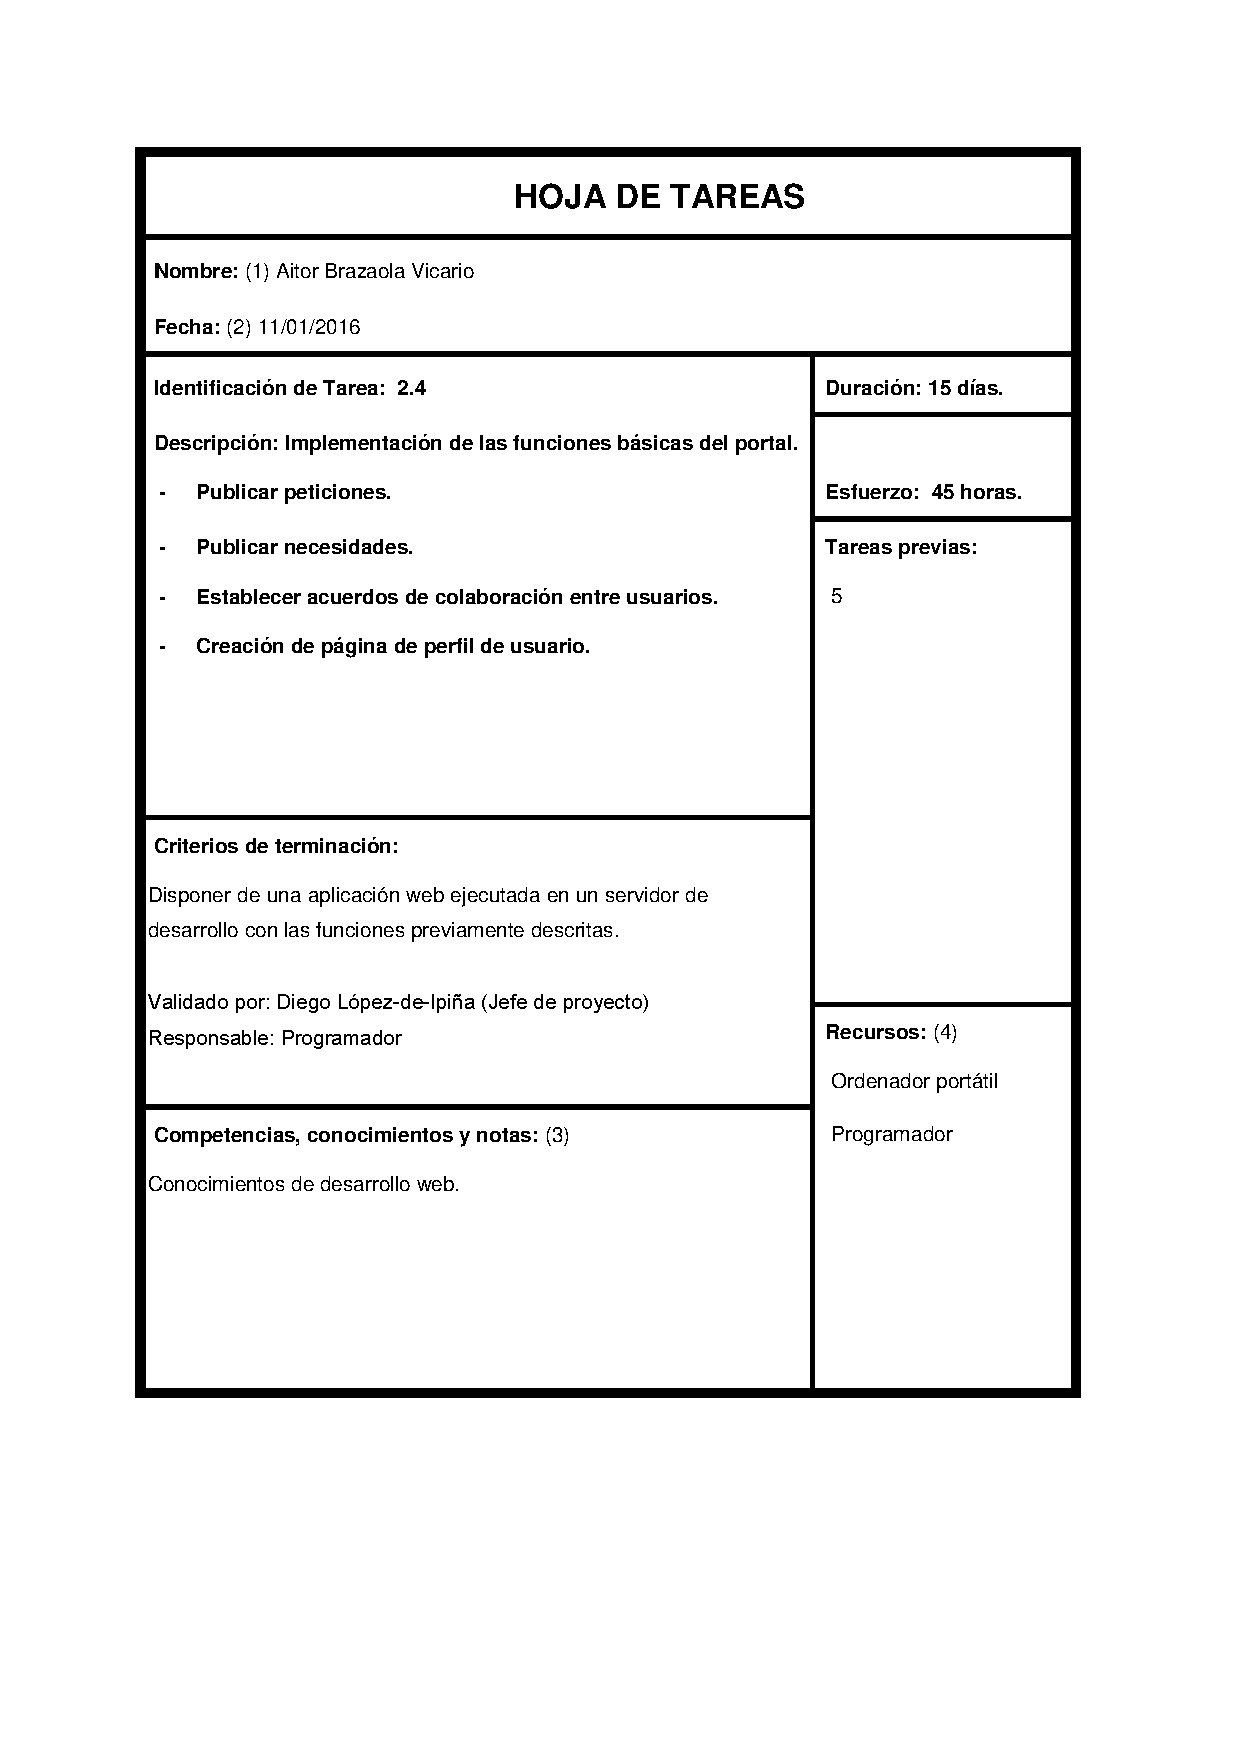
\includegraphics[width=0.9\textwidth]{fig/Tareas/24}
	\caption{Tarea 2.4.}
	\label{fig:t24}
\end{figure}

\begin{figure}[H]
	\centering
	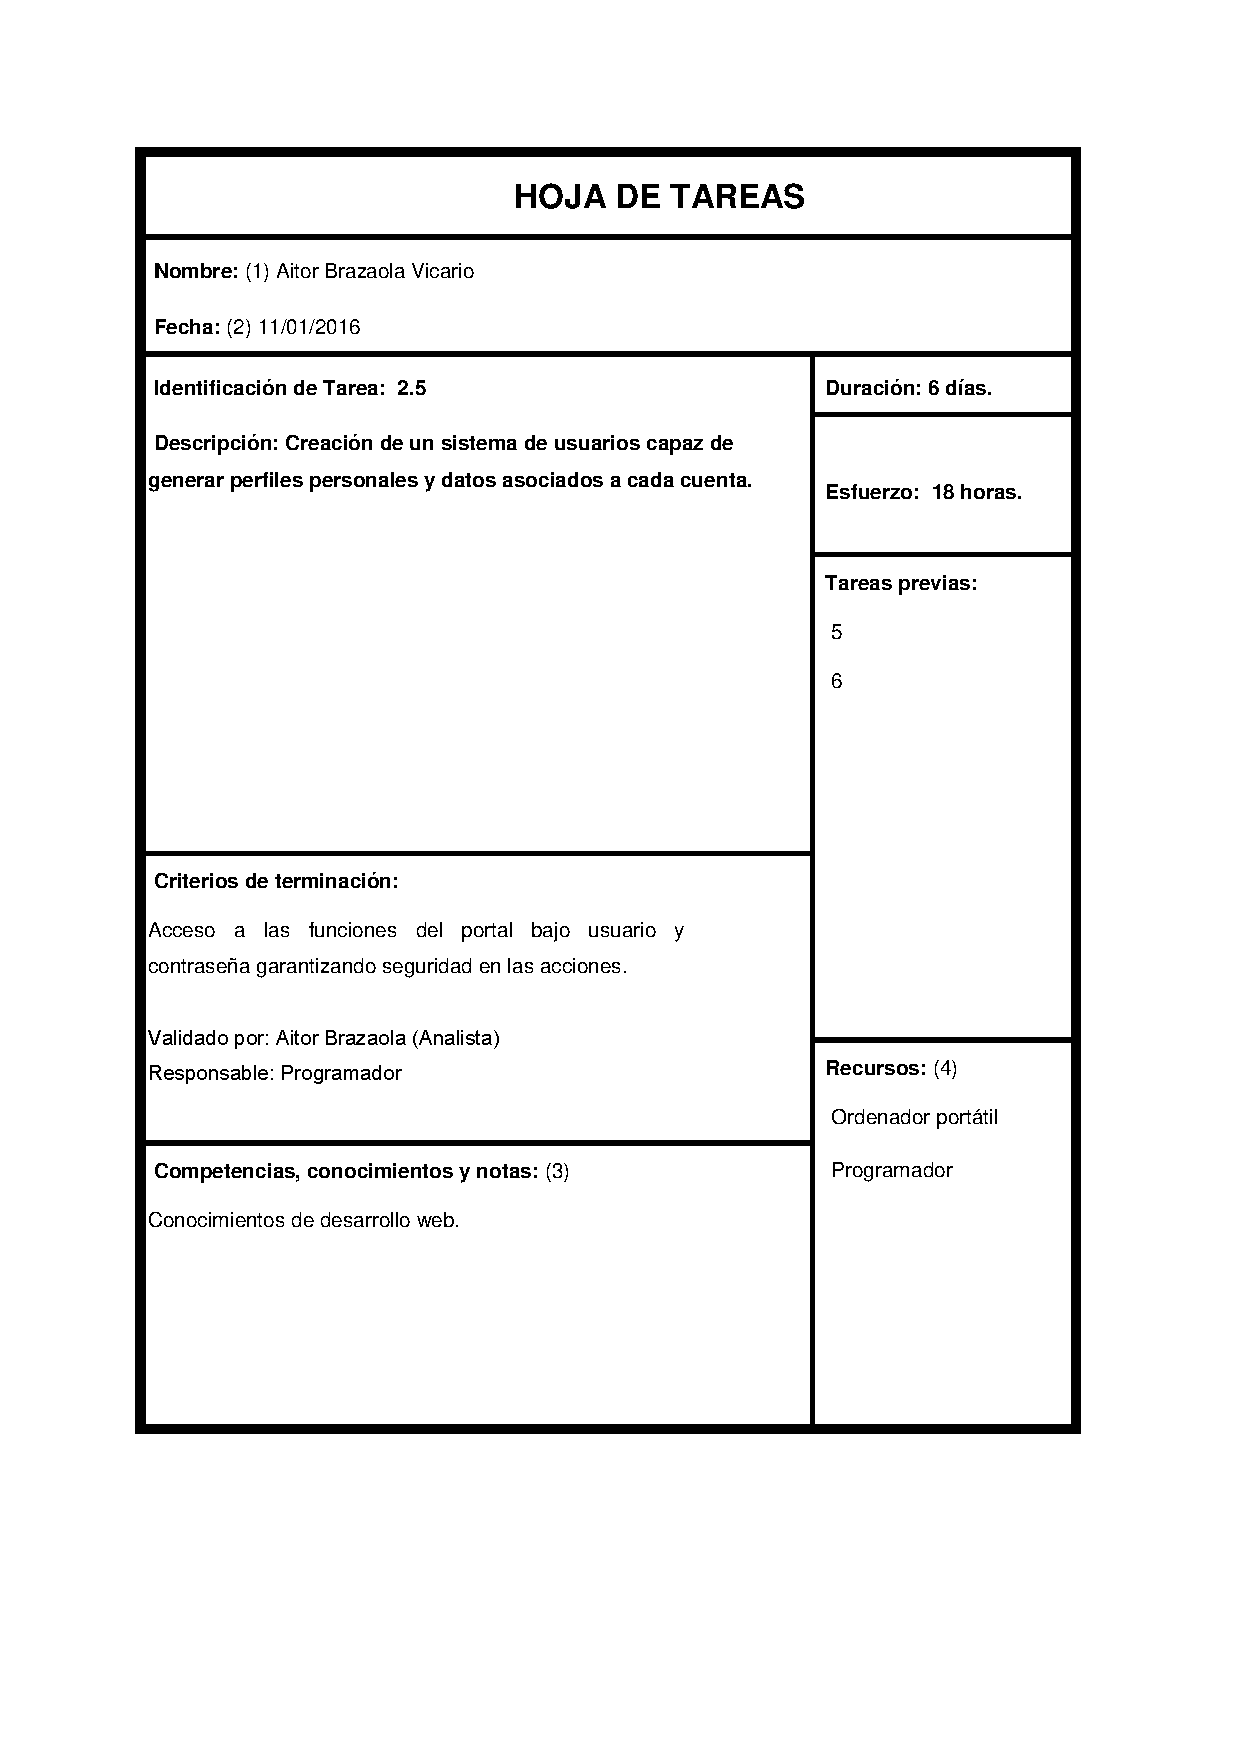
\includegraphics[width=0.9\textwidth]{fig/Tareas/25}
	\caption{Tarea 2.5.}
	\label{fig:t25}
\end{figure}

\begin{figure}[H]
	\centering
	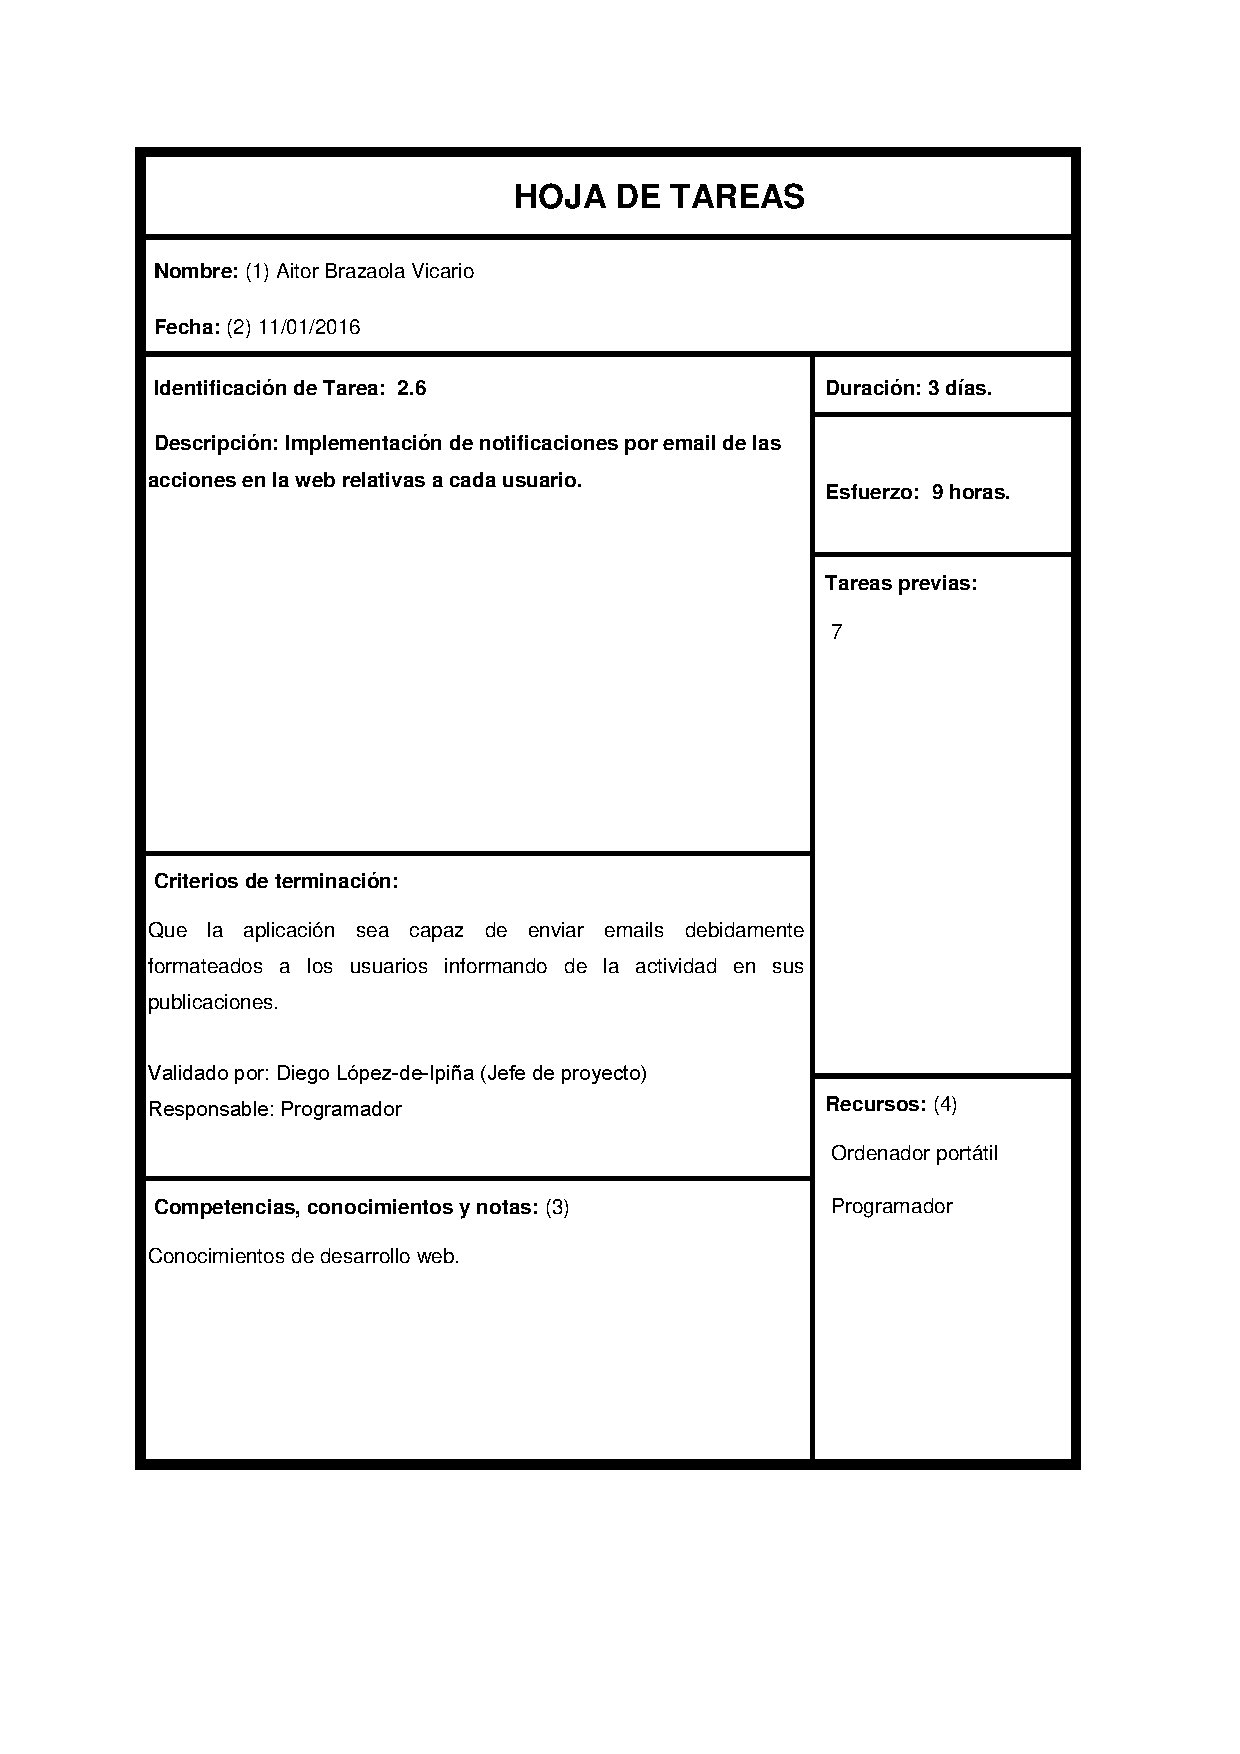
\includegraphics[width=0.9\textwidth]{fig/Tareas/26}
	\caption{Tarea 2.6.}
	\label{fig:t26}
\end{figure}

\begin{figure}[H]
	\centering
	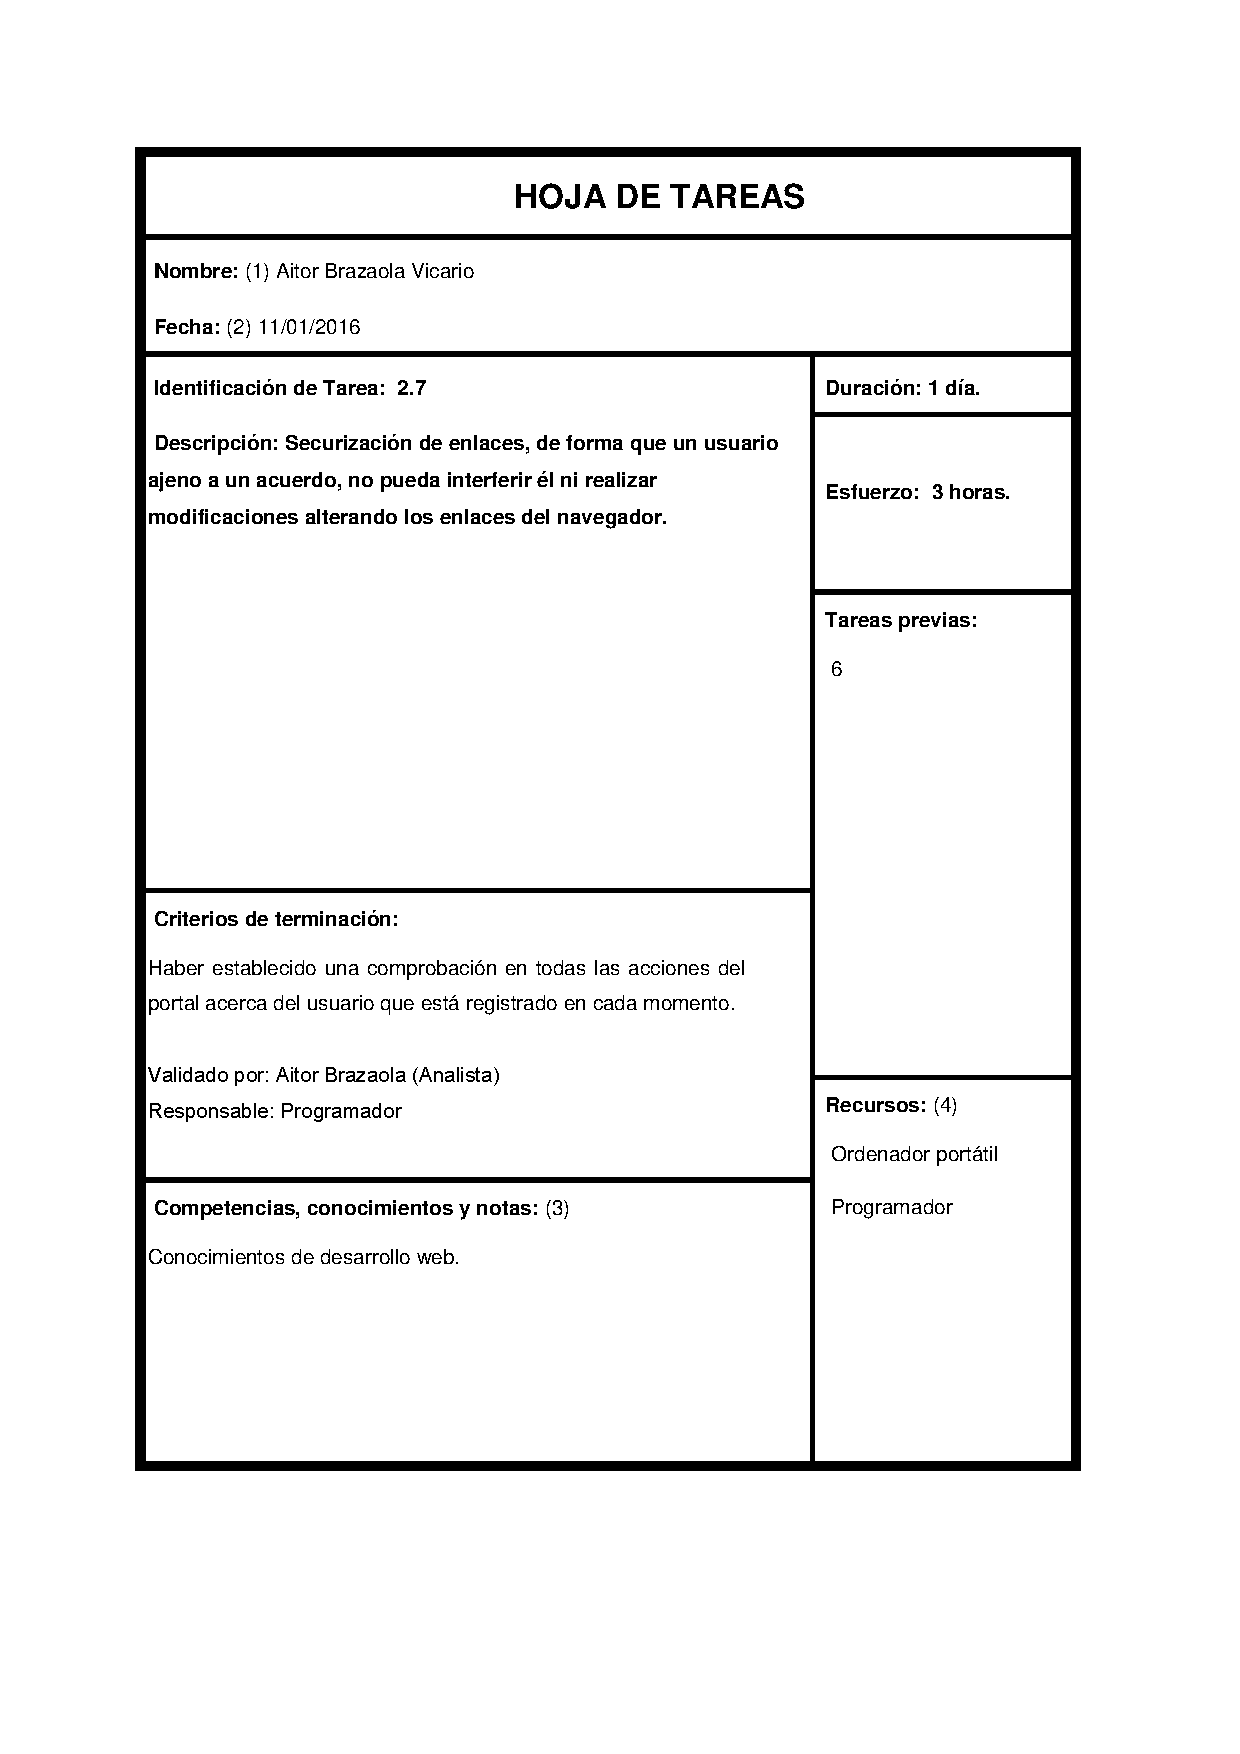
\includegraphics[width=0.9\textwidth]{fig/Tareas/27}
	\caption{Tarea 2.7.}
	\label{fig:t27}
\end{figure}

\begin{figure}[H]
	\centering
	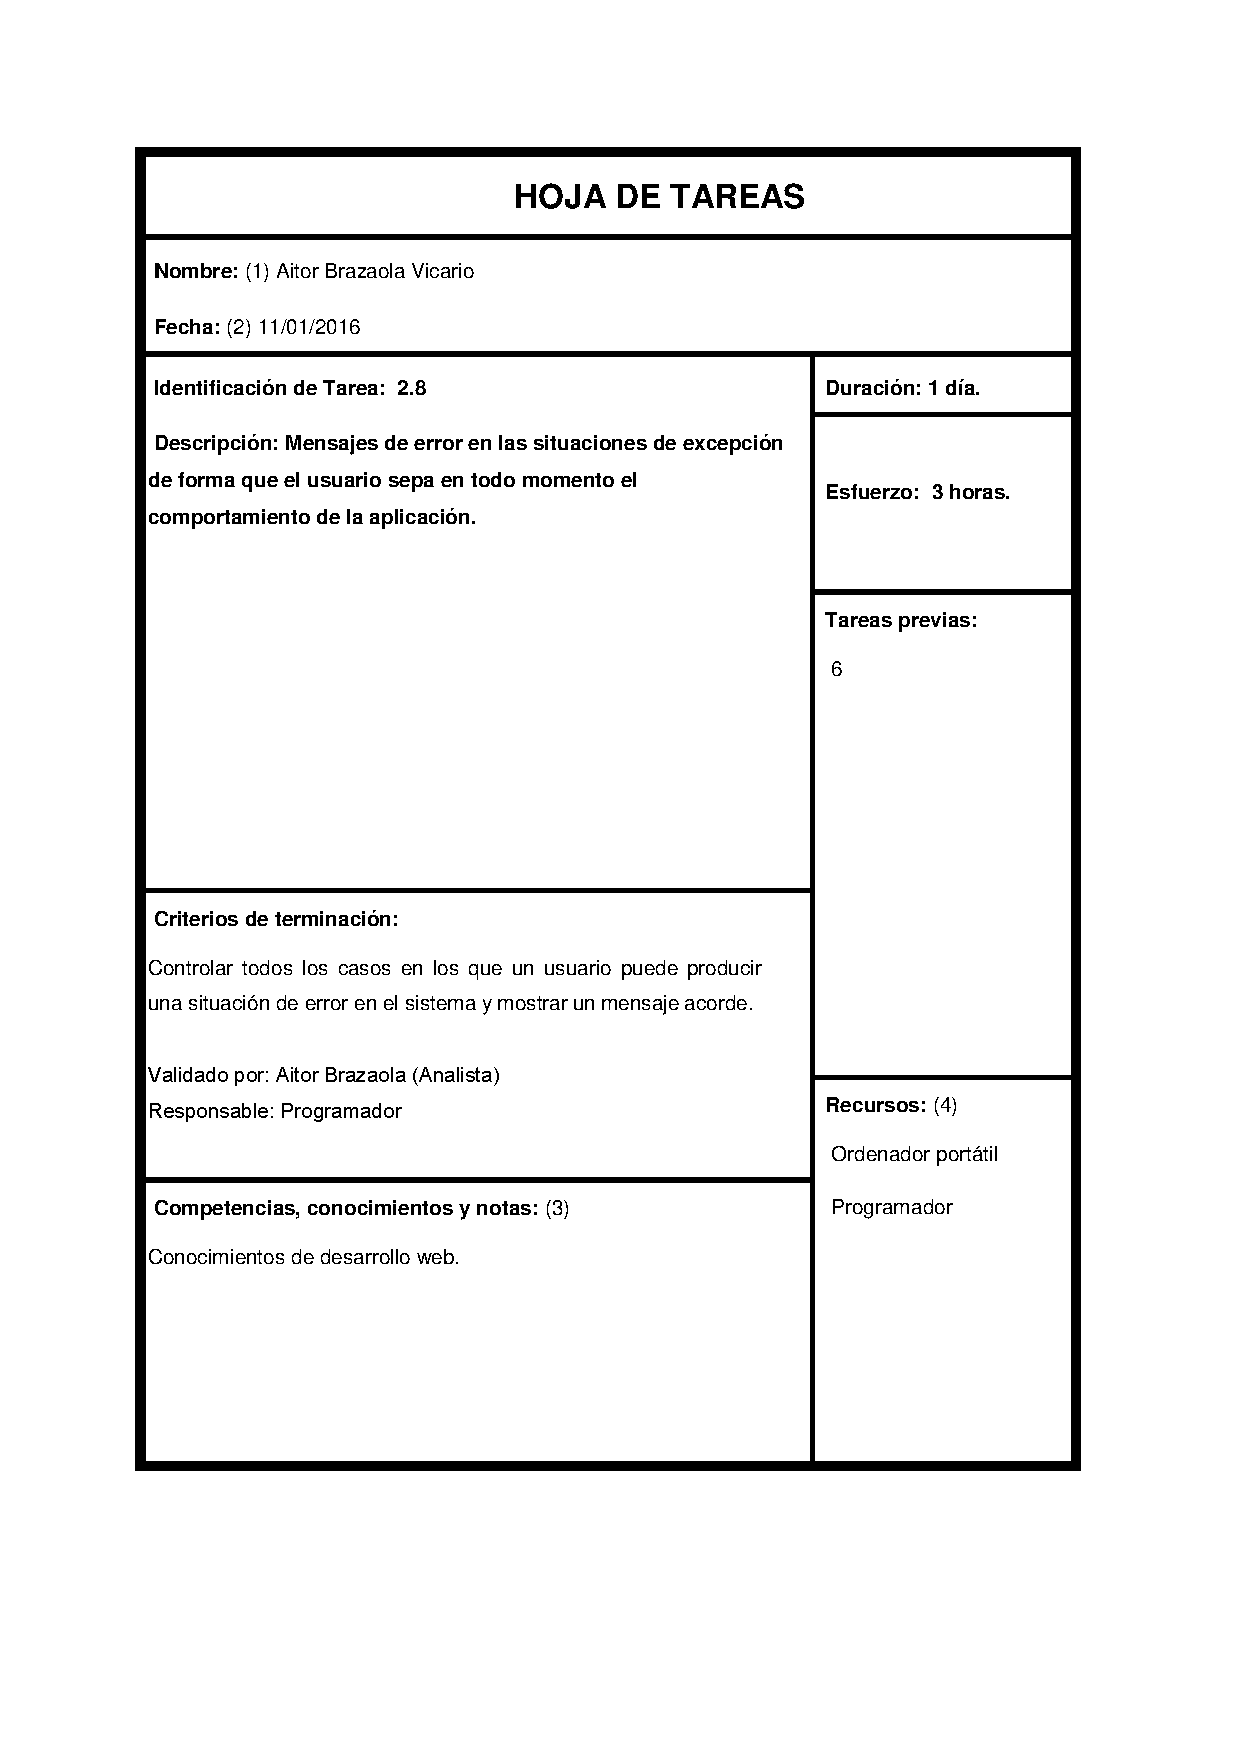
\includegraphics[width=0.9\textwidth]{fig/Tareas/28}
	\caption{Tarea 2.8.}
	\label{fig:t28}
\end{figure}

\begin{figure}[H]
	\centering
	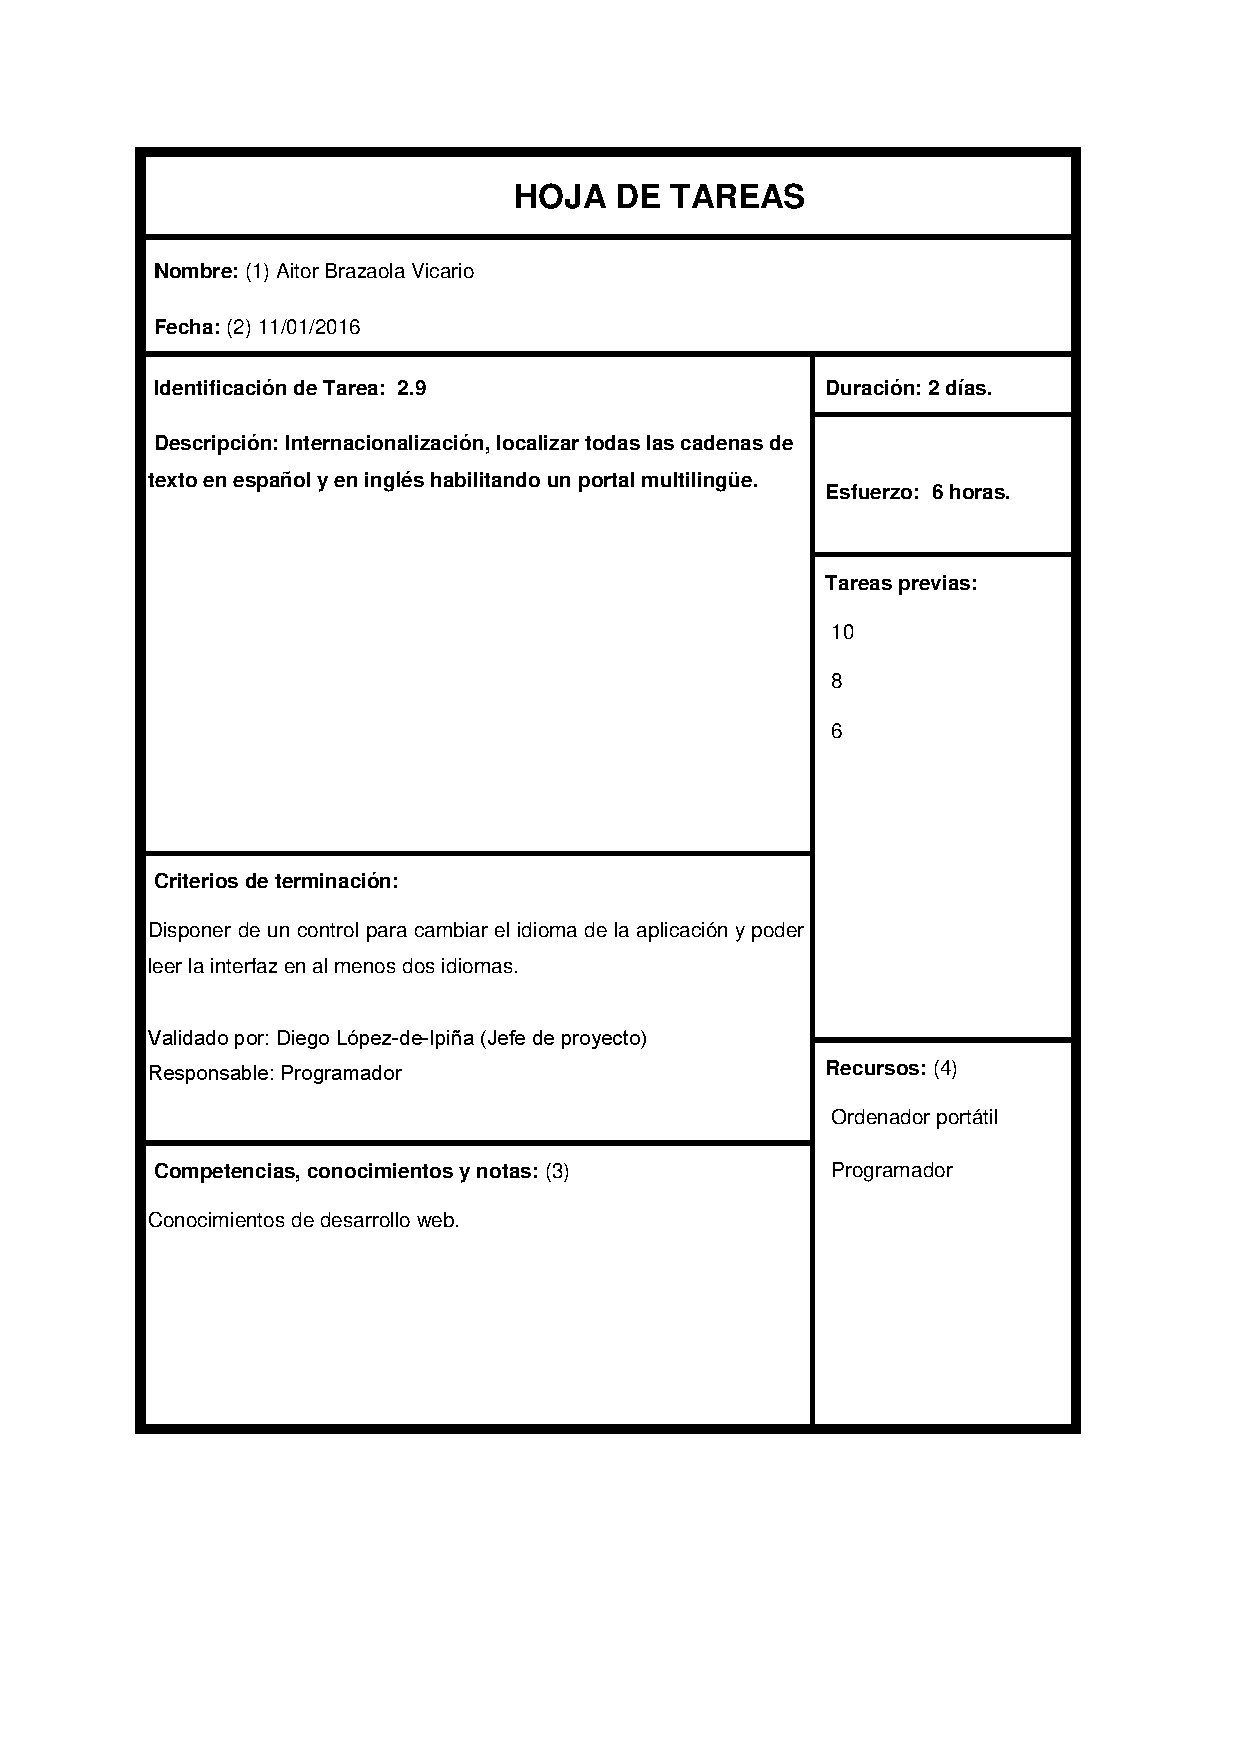
\includegraphics[width=0.9\textwidth]{fig/Tareas/29}
	\caption{Tarea 2.9.}
	\label{fig:t29}
\end{figure}

\begin{figure}[H]
	\centering
	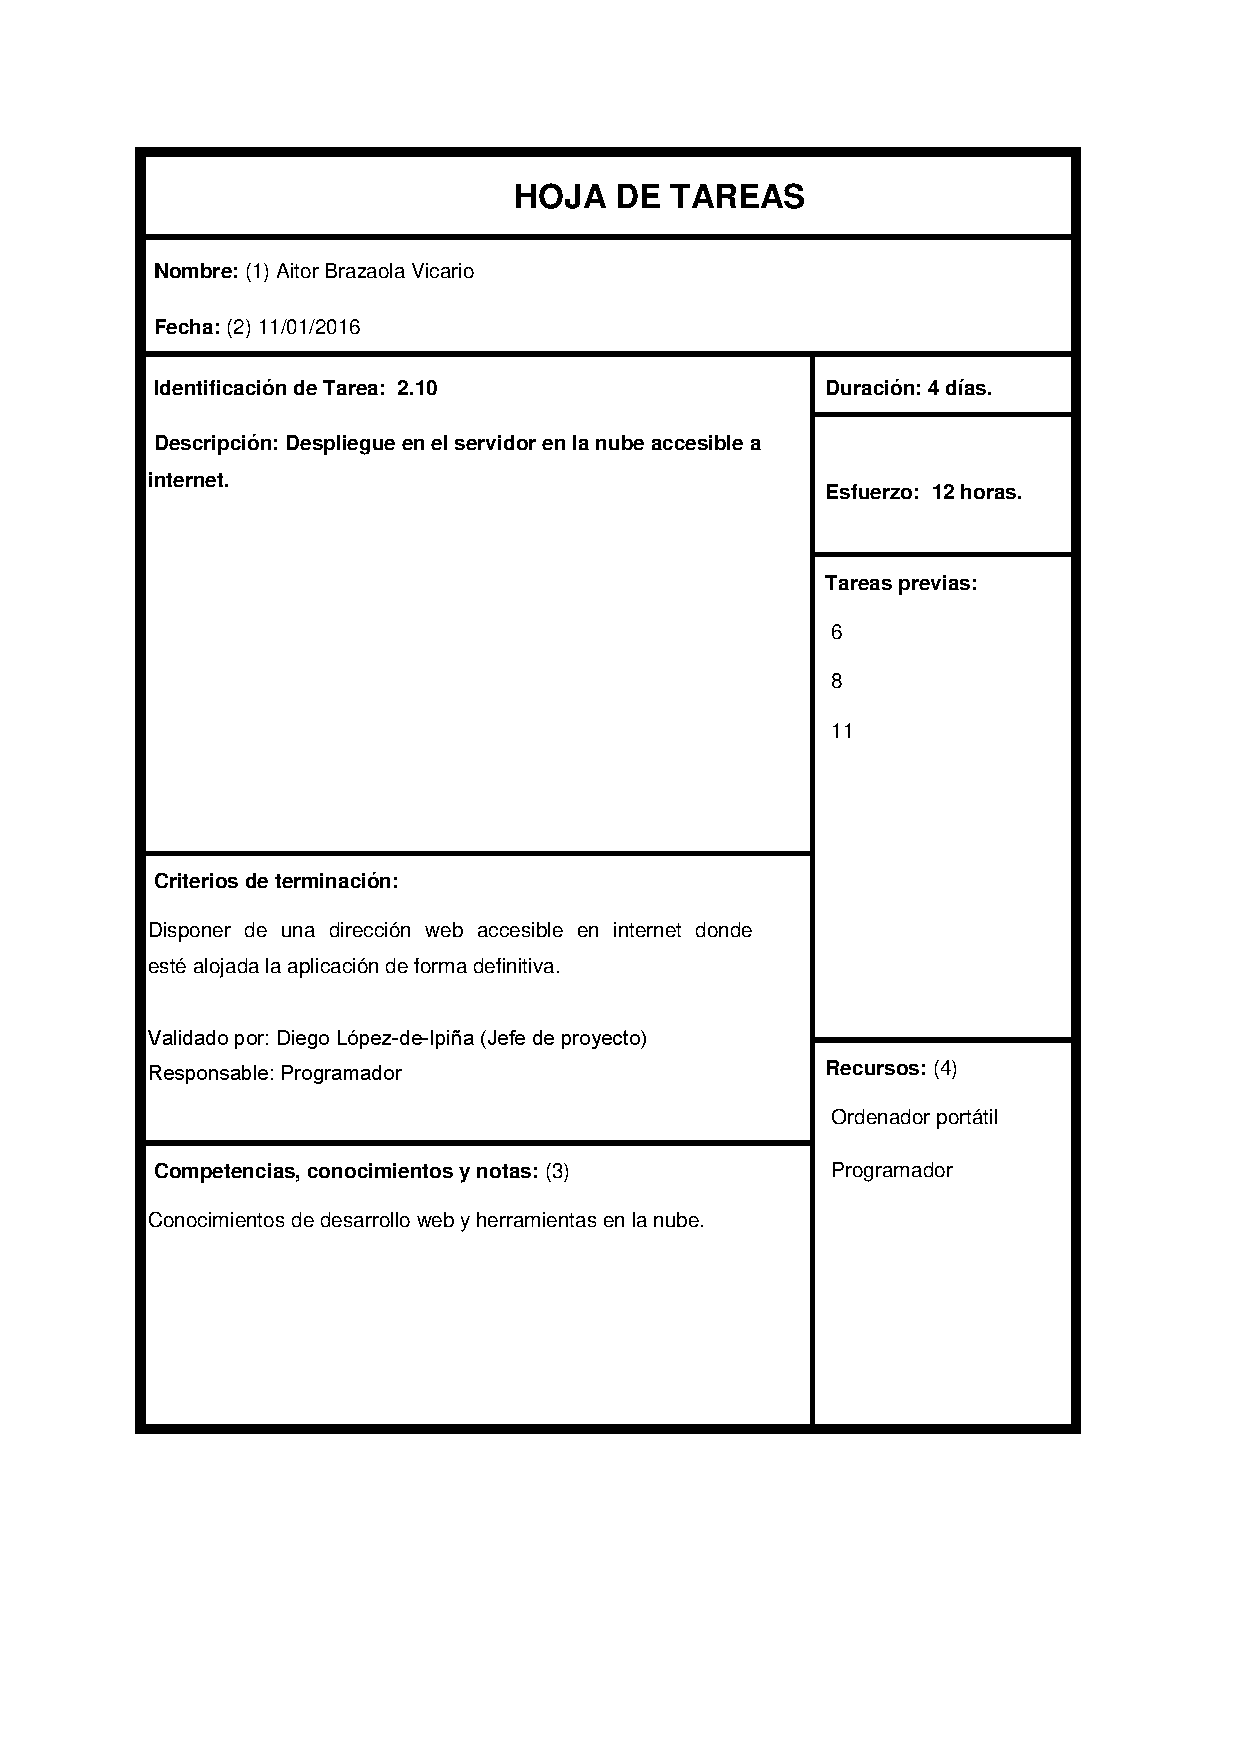
\includegraphics[width=0.9\textwidth]{fig/Tareas/210}
	\caption{Tarea 2.10.}
	\label{fig:t210}
\end{figure}

\begin{figure}[H]
	\centering
	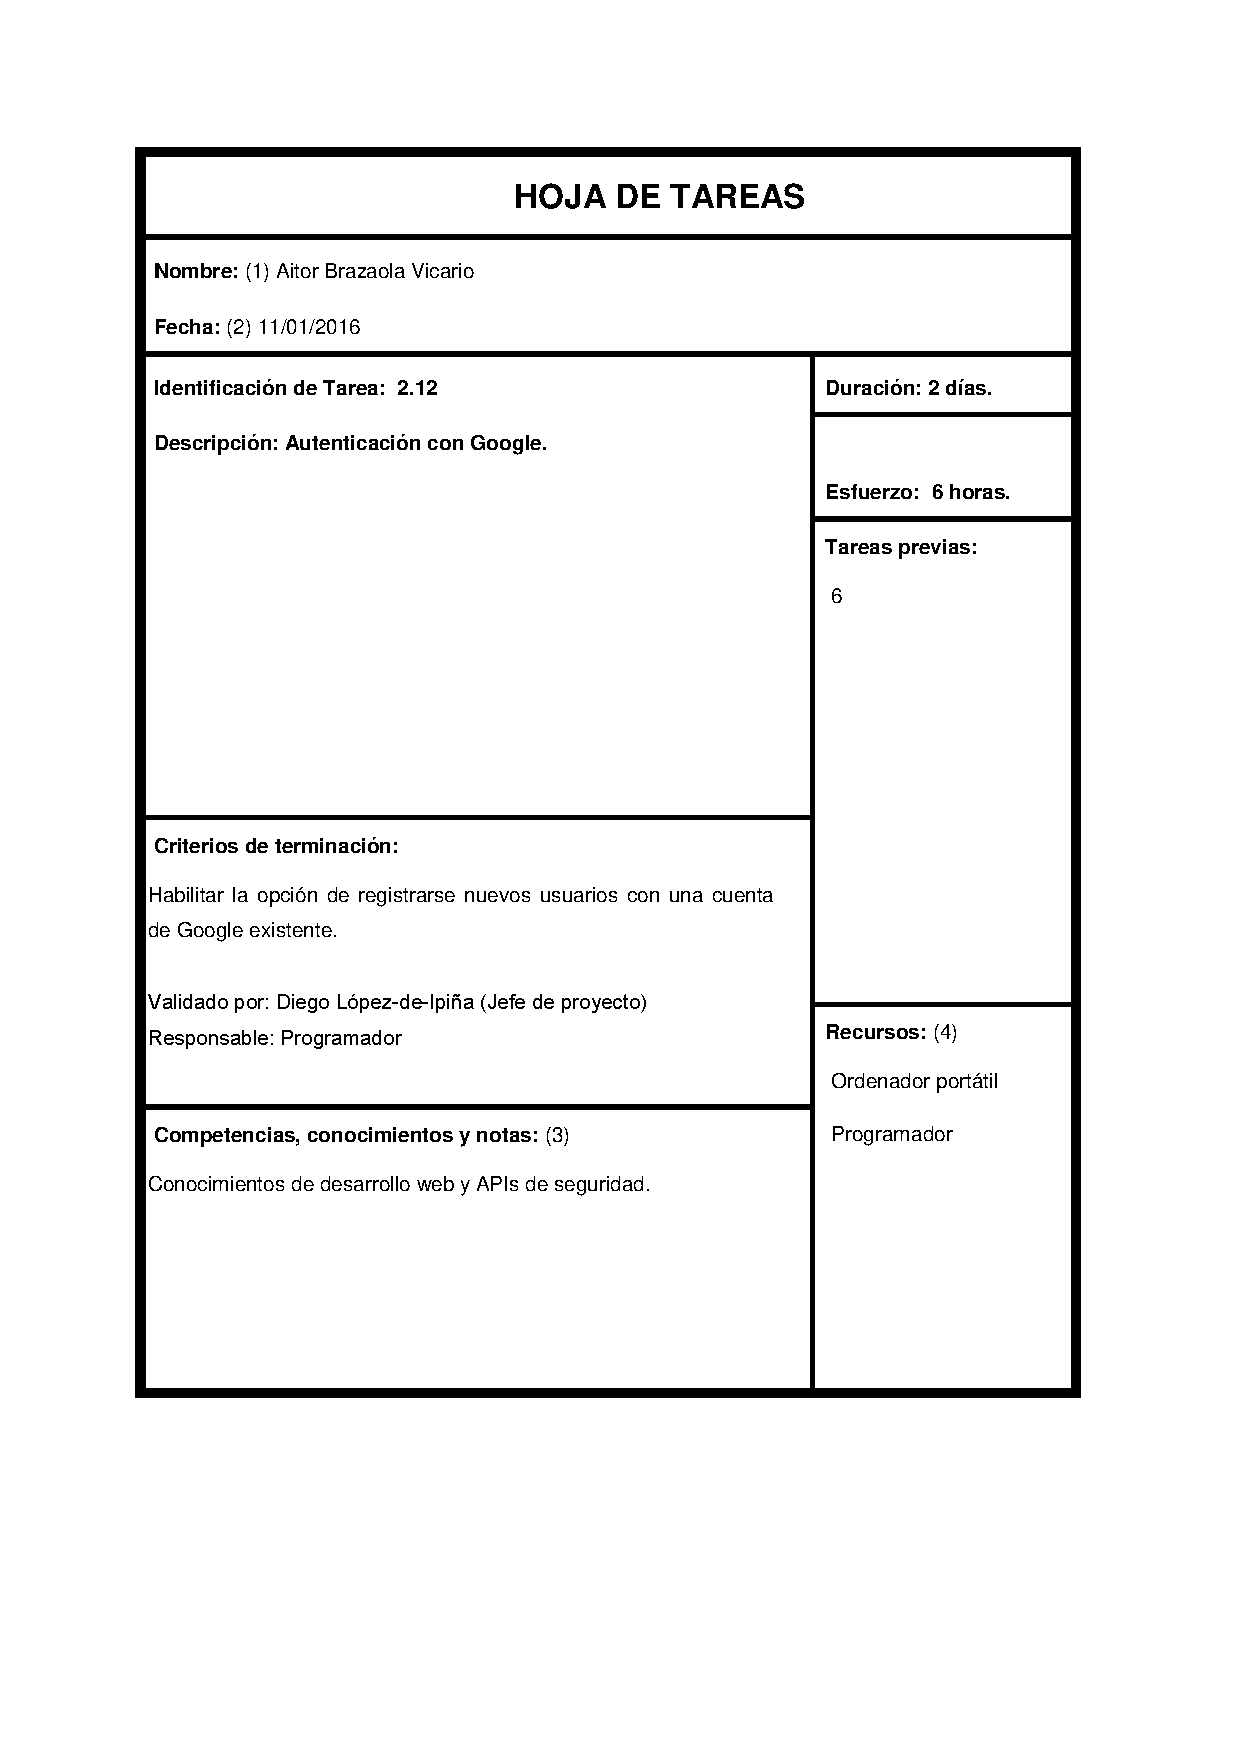
\includegraphics[width=0.9\textwidth]{fig/Tareas/212}
	\caption{Tarea 2.12.}
	\label{fig:t212}
\end{figure}

\begin{figure}[H]
	\centering
	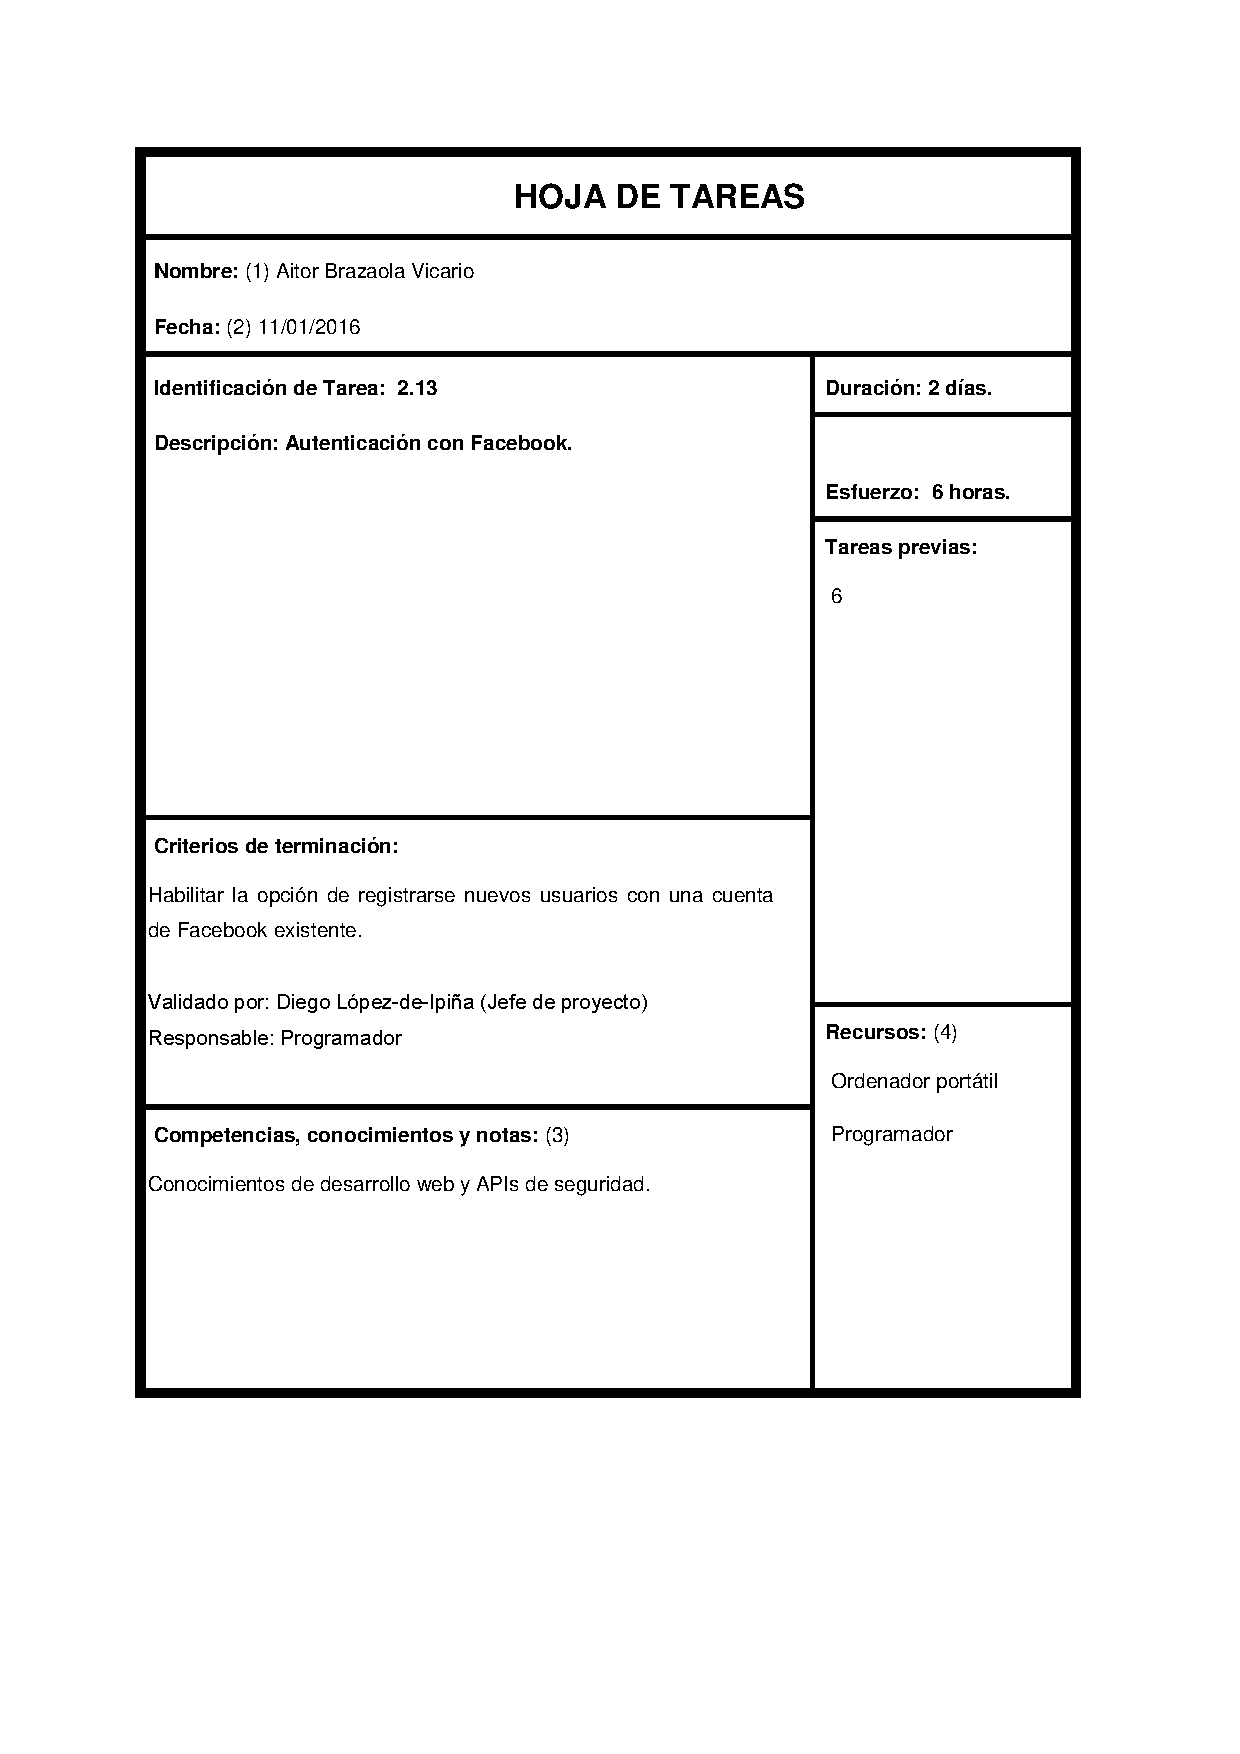
\includegraphics[width=0.9\textwidth]{fig/Tareas/213}
	\caption{Tarea 2.13.}
	\label{fig:t213}
\end{figure}

\begin{figure}[H]
	\centering
	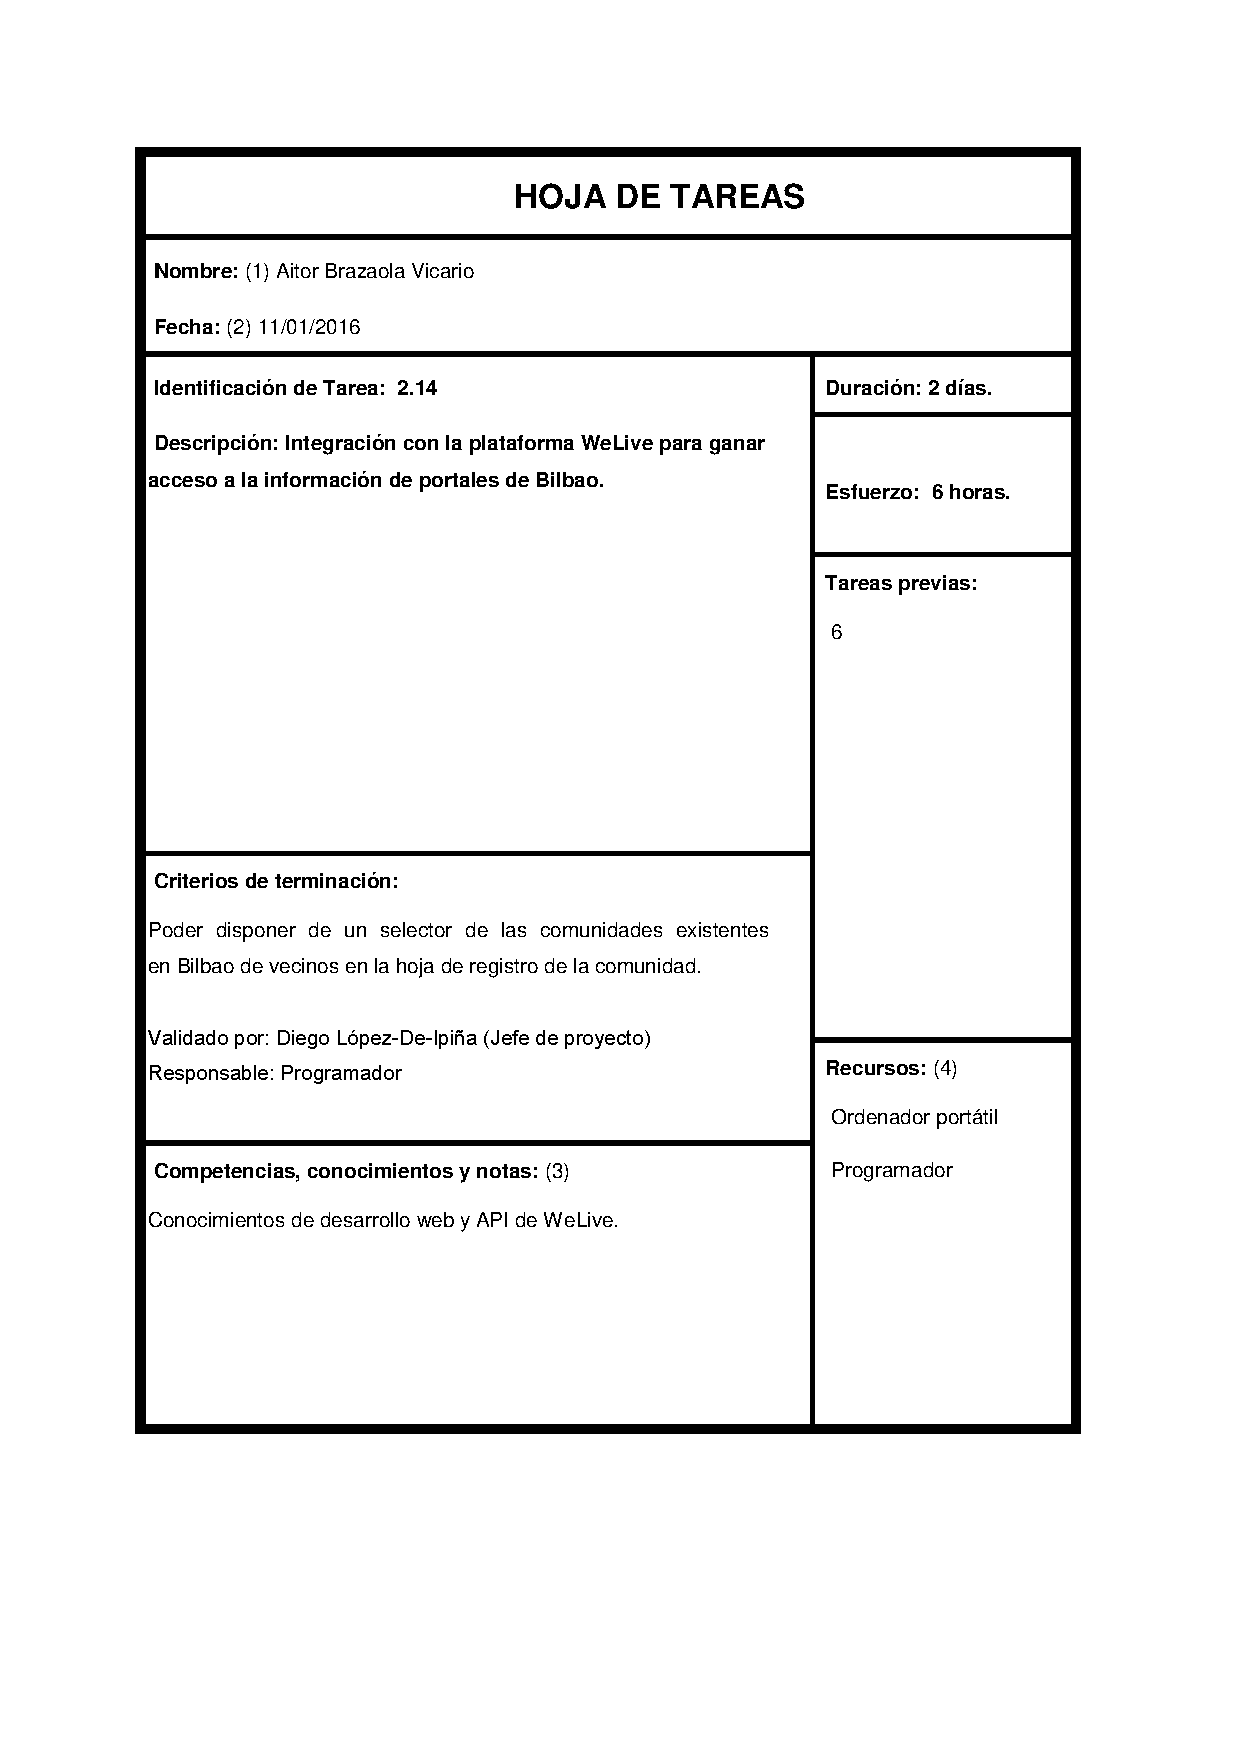
\includegraphics[width=0.9\textwidth]{fig/Tareas/214}
	\caption{Tarea 2.14.}
	\label{fig:t214}
\end{figure}

\begin{figure}[H]
	\centering
	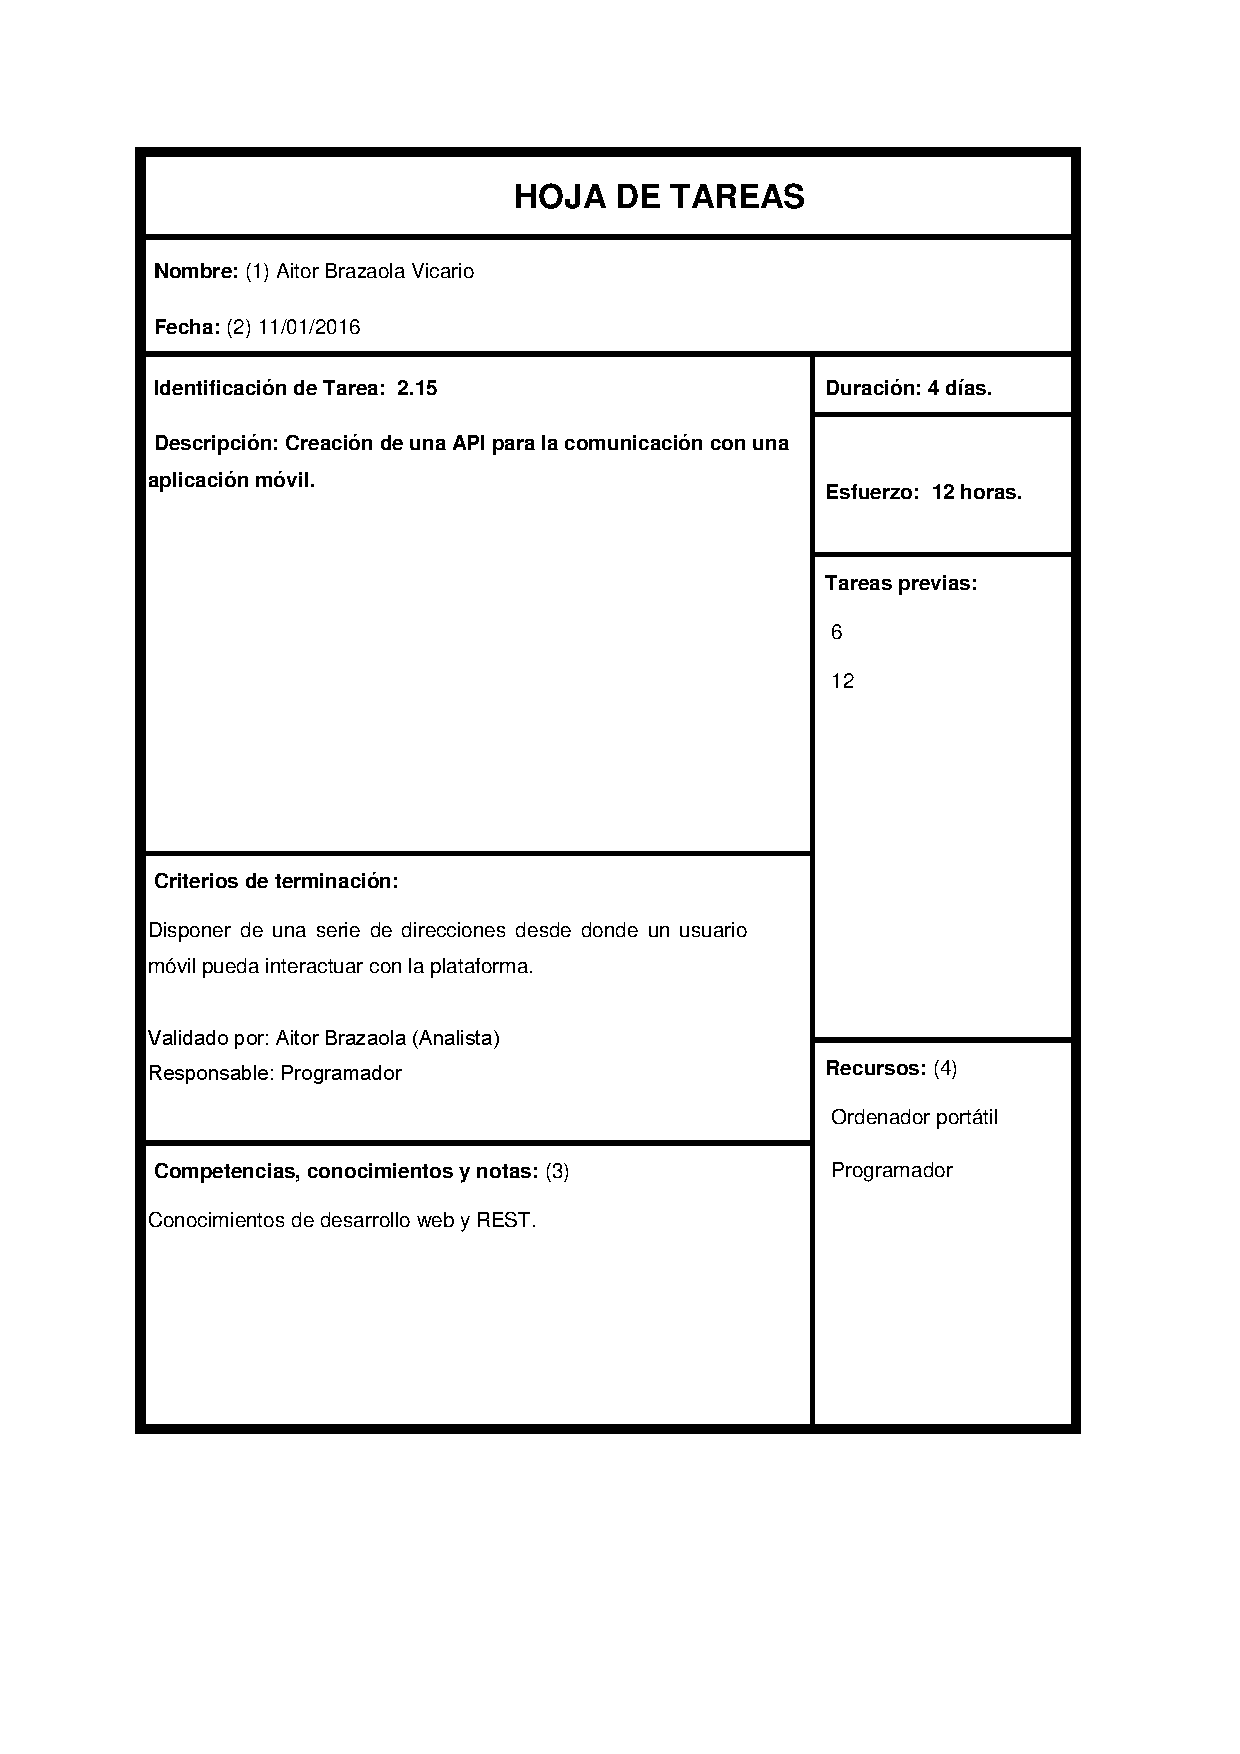
\includegraphics[width=0.9\textwidth]{fig/Tareas/215}
	\caption{Tarea 2.15.}
	\label{fig:t215}
\end{figure}

\begin{figure}[H]
	\centering
	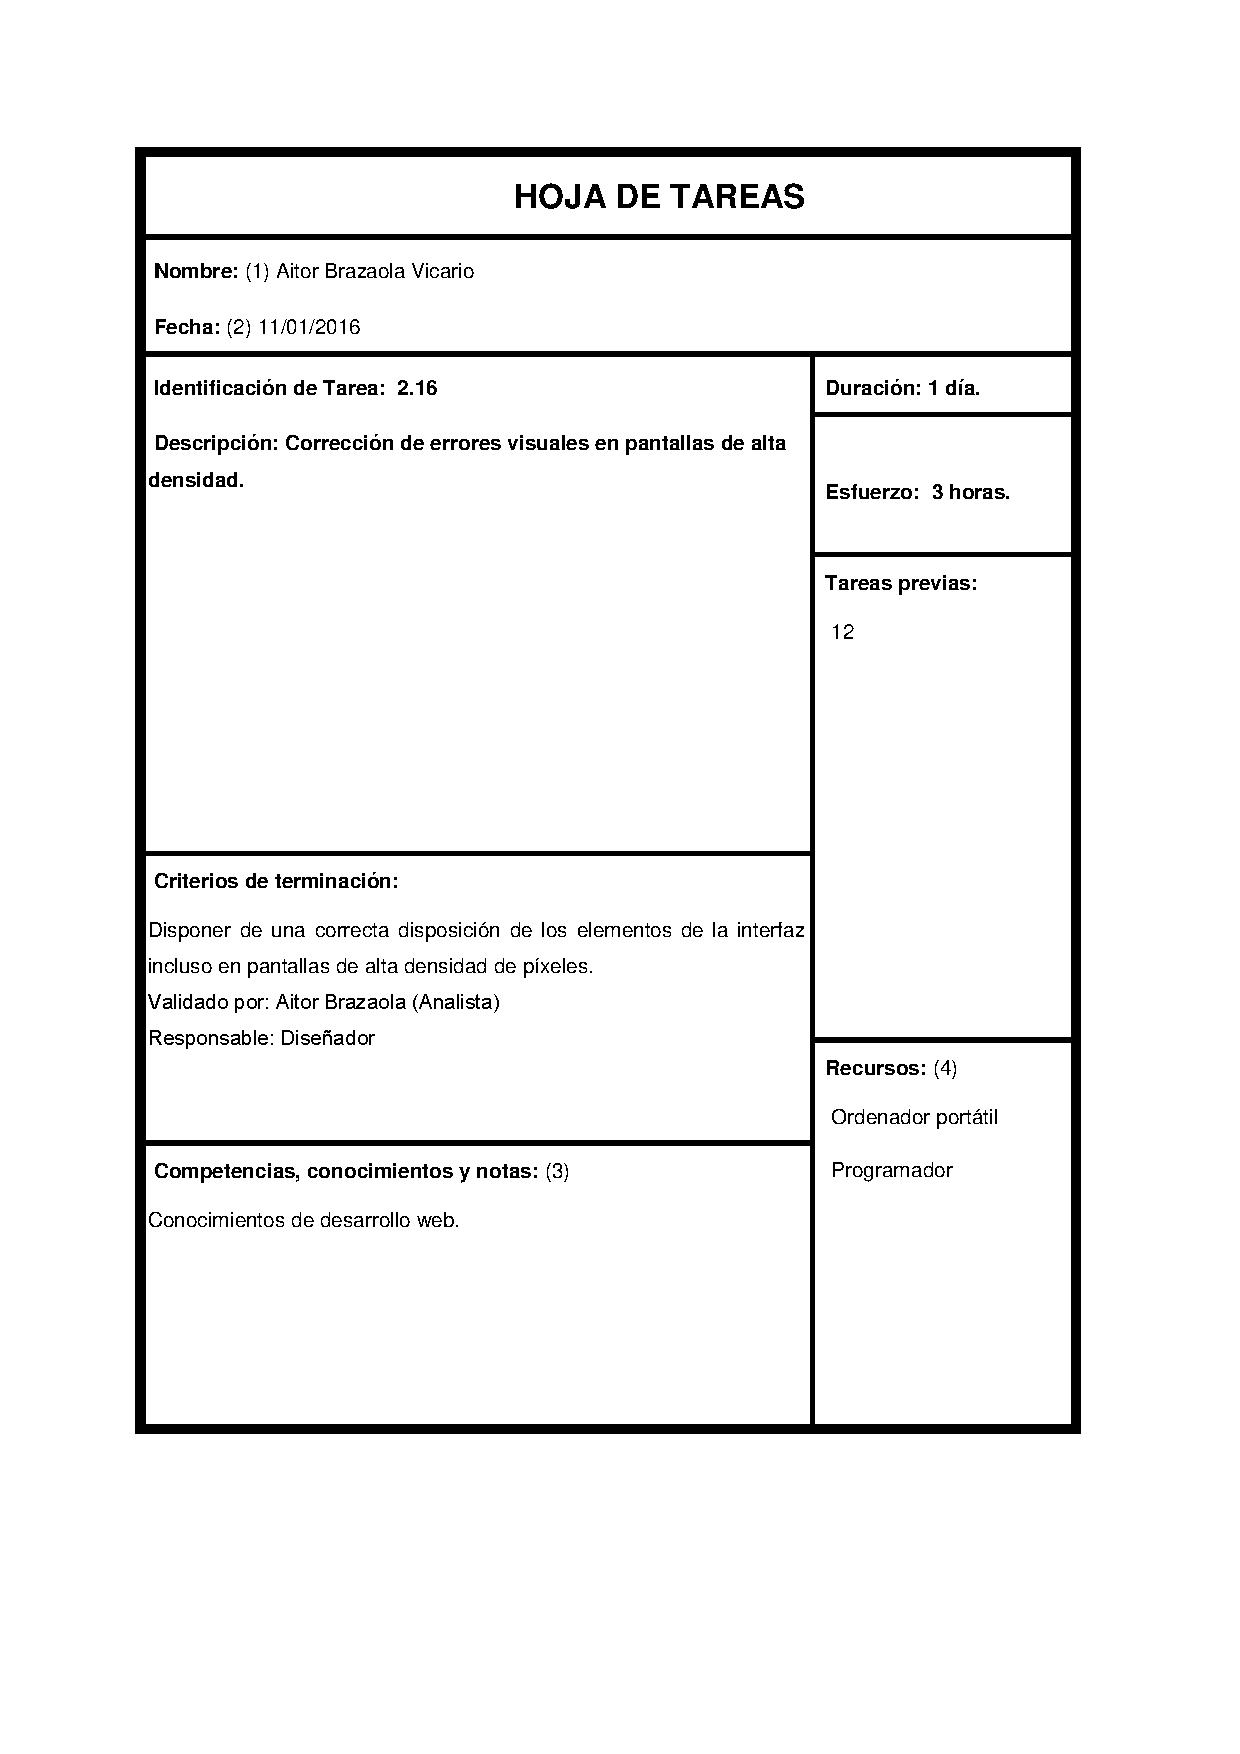
\includegraphics[width=0.9\textwidth]{fig/Tareas/216}
	\caption{Tarea 2.16.}
	\label{fig:t216}
\end{figure}

\begin{figure}[H]
	\centering
	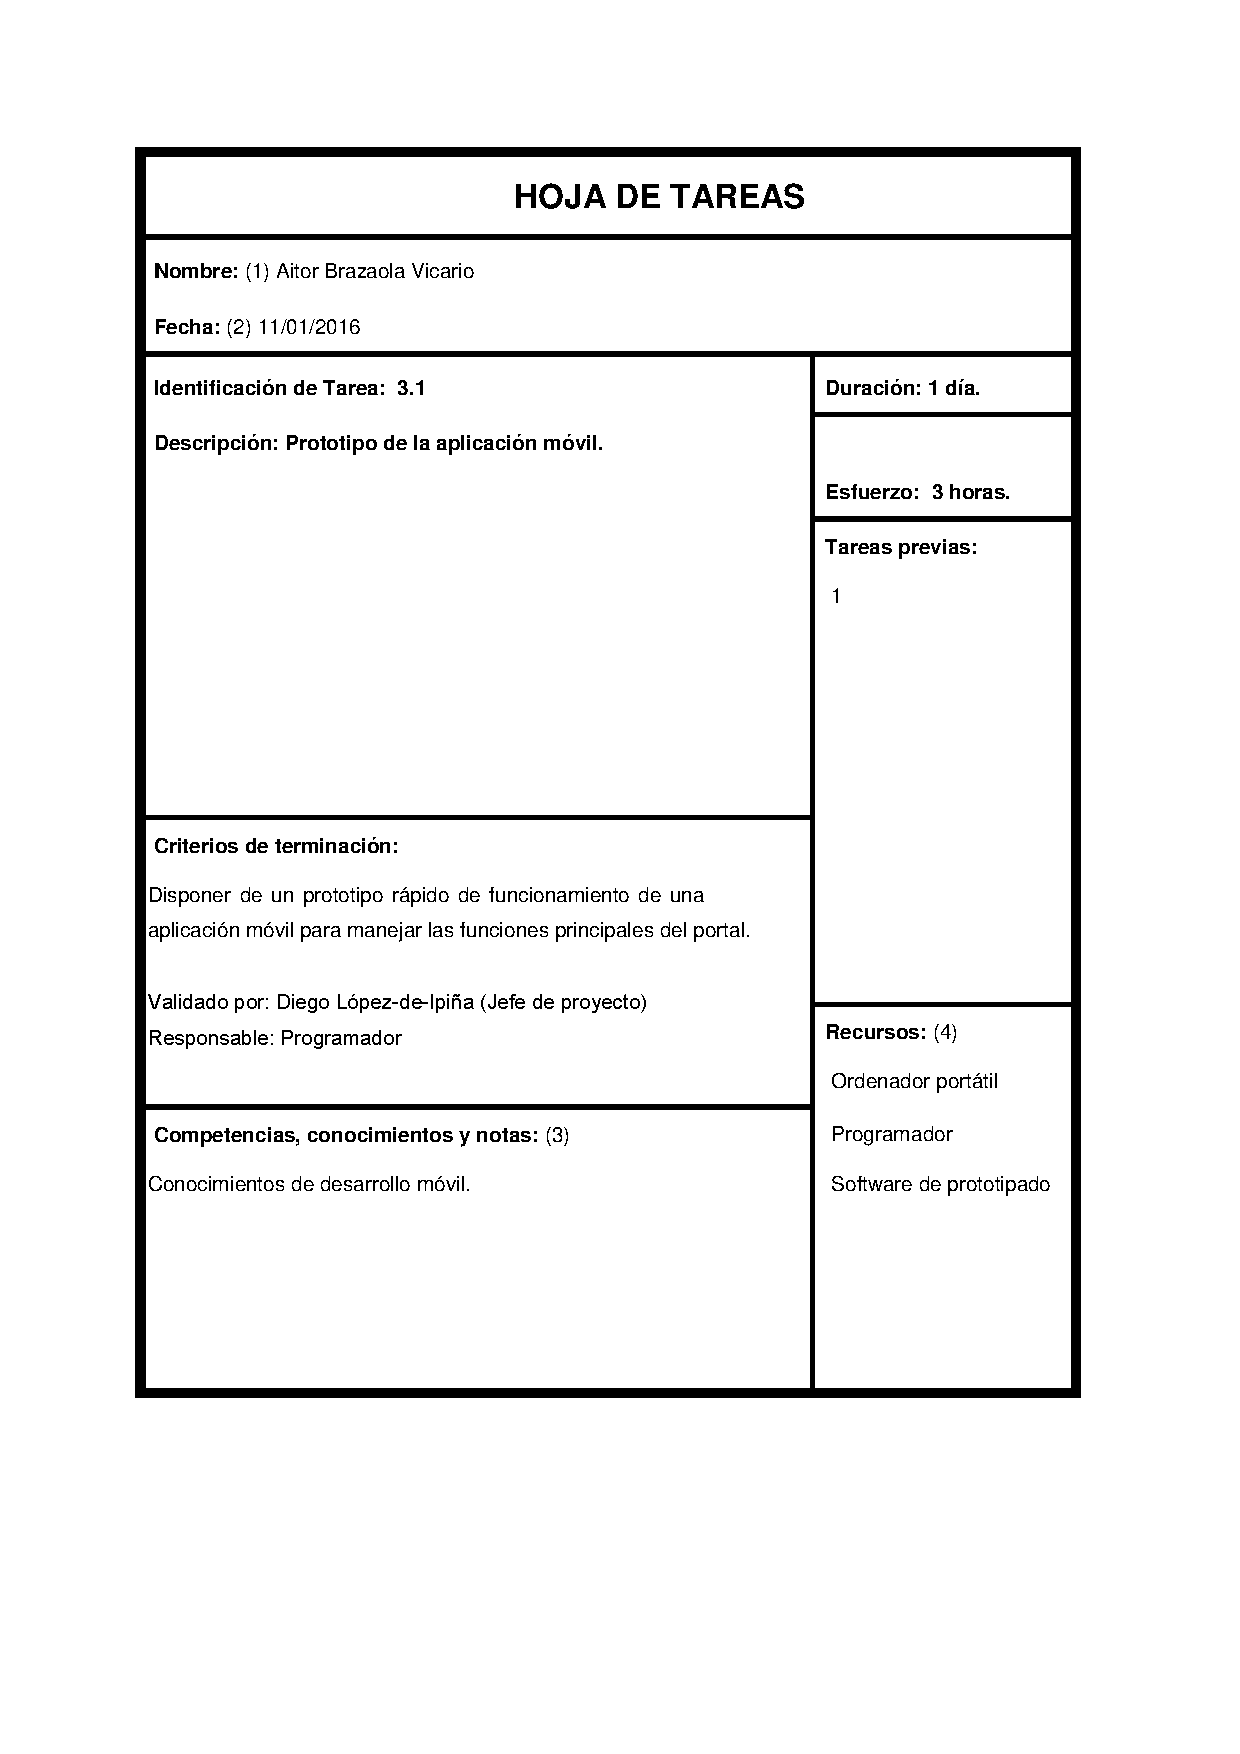
\includegraphics[width=0.9\textwidth]{fig/Tareas/31}
	\caption{Tarea 3.1.}
	\label{fig:t31}
\end{figure}

\begin{figure}[H]
	\centering
	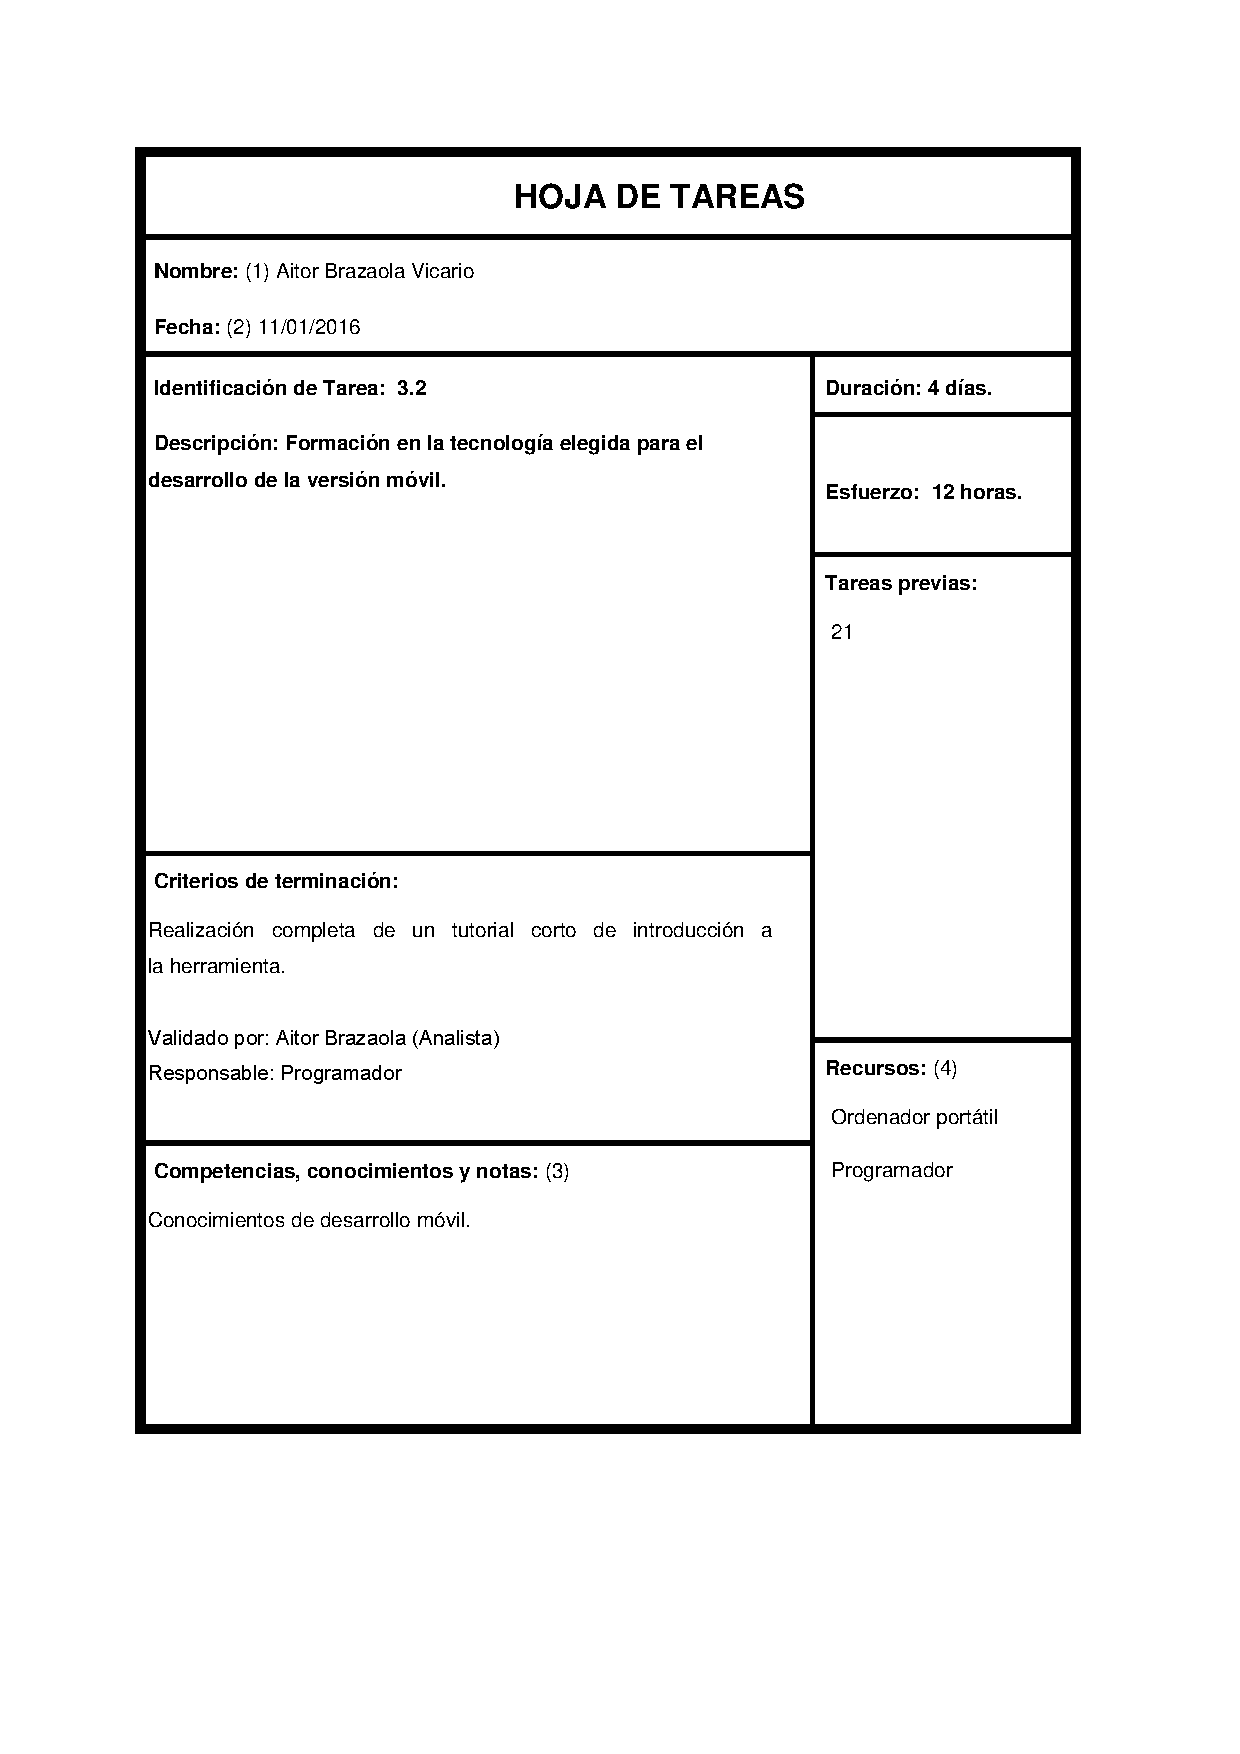
\includegraphics[width=0.9\textwidth]{fig/Tareas/32}
	\caption{Tarea 3.2.}
	\label{fig:t32}
\end{figure}

\begin{figure}[H]
	\centering
	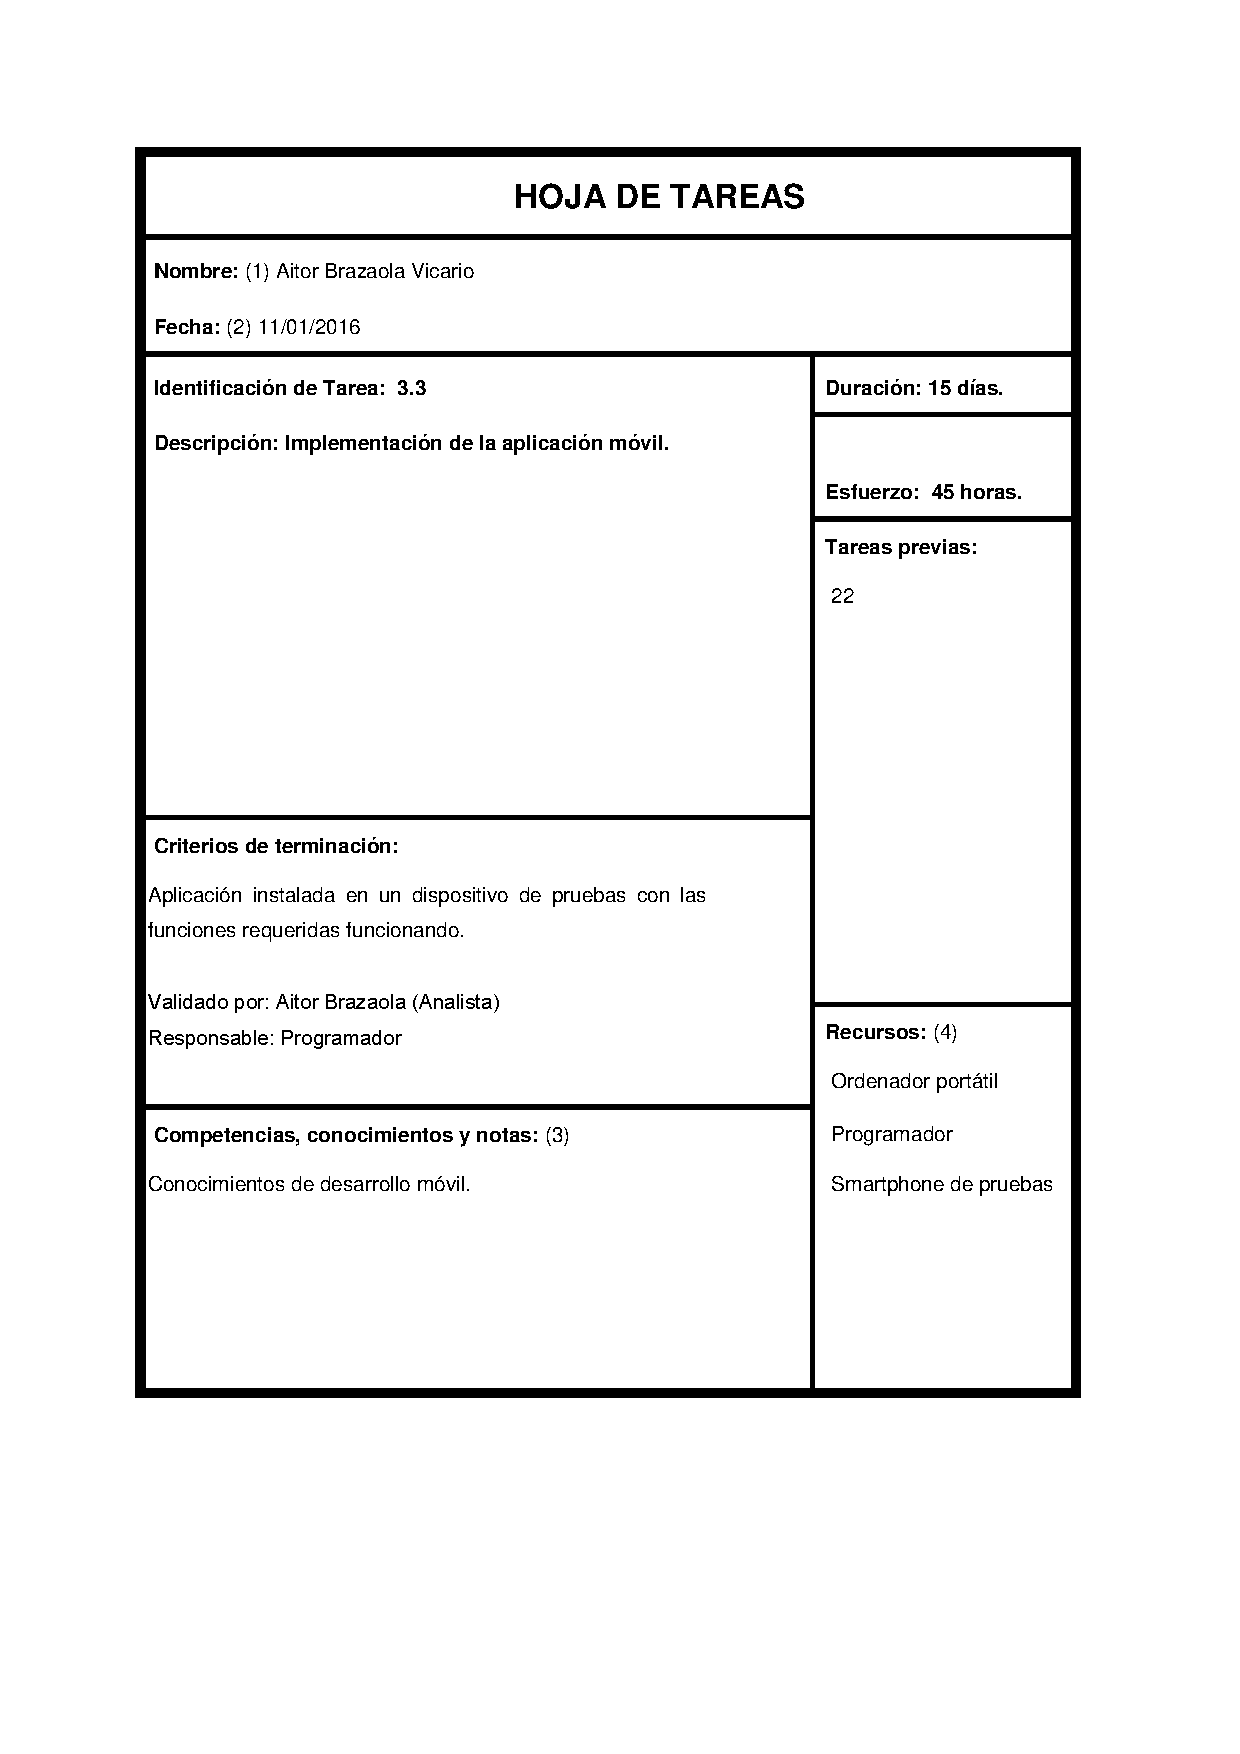
\includegraphics[width=0.9\textwidth]{fig/Tareas/33}
	\caption{Tarea 3.3.}
	\label{fig:t33}
\end{figure}

\begin{figure}[H]
	\centering
	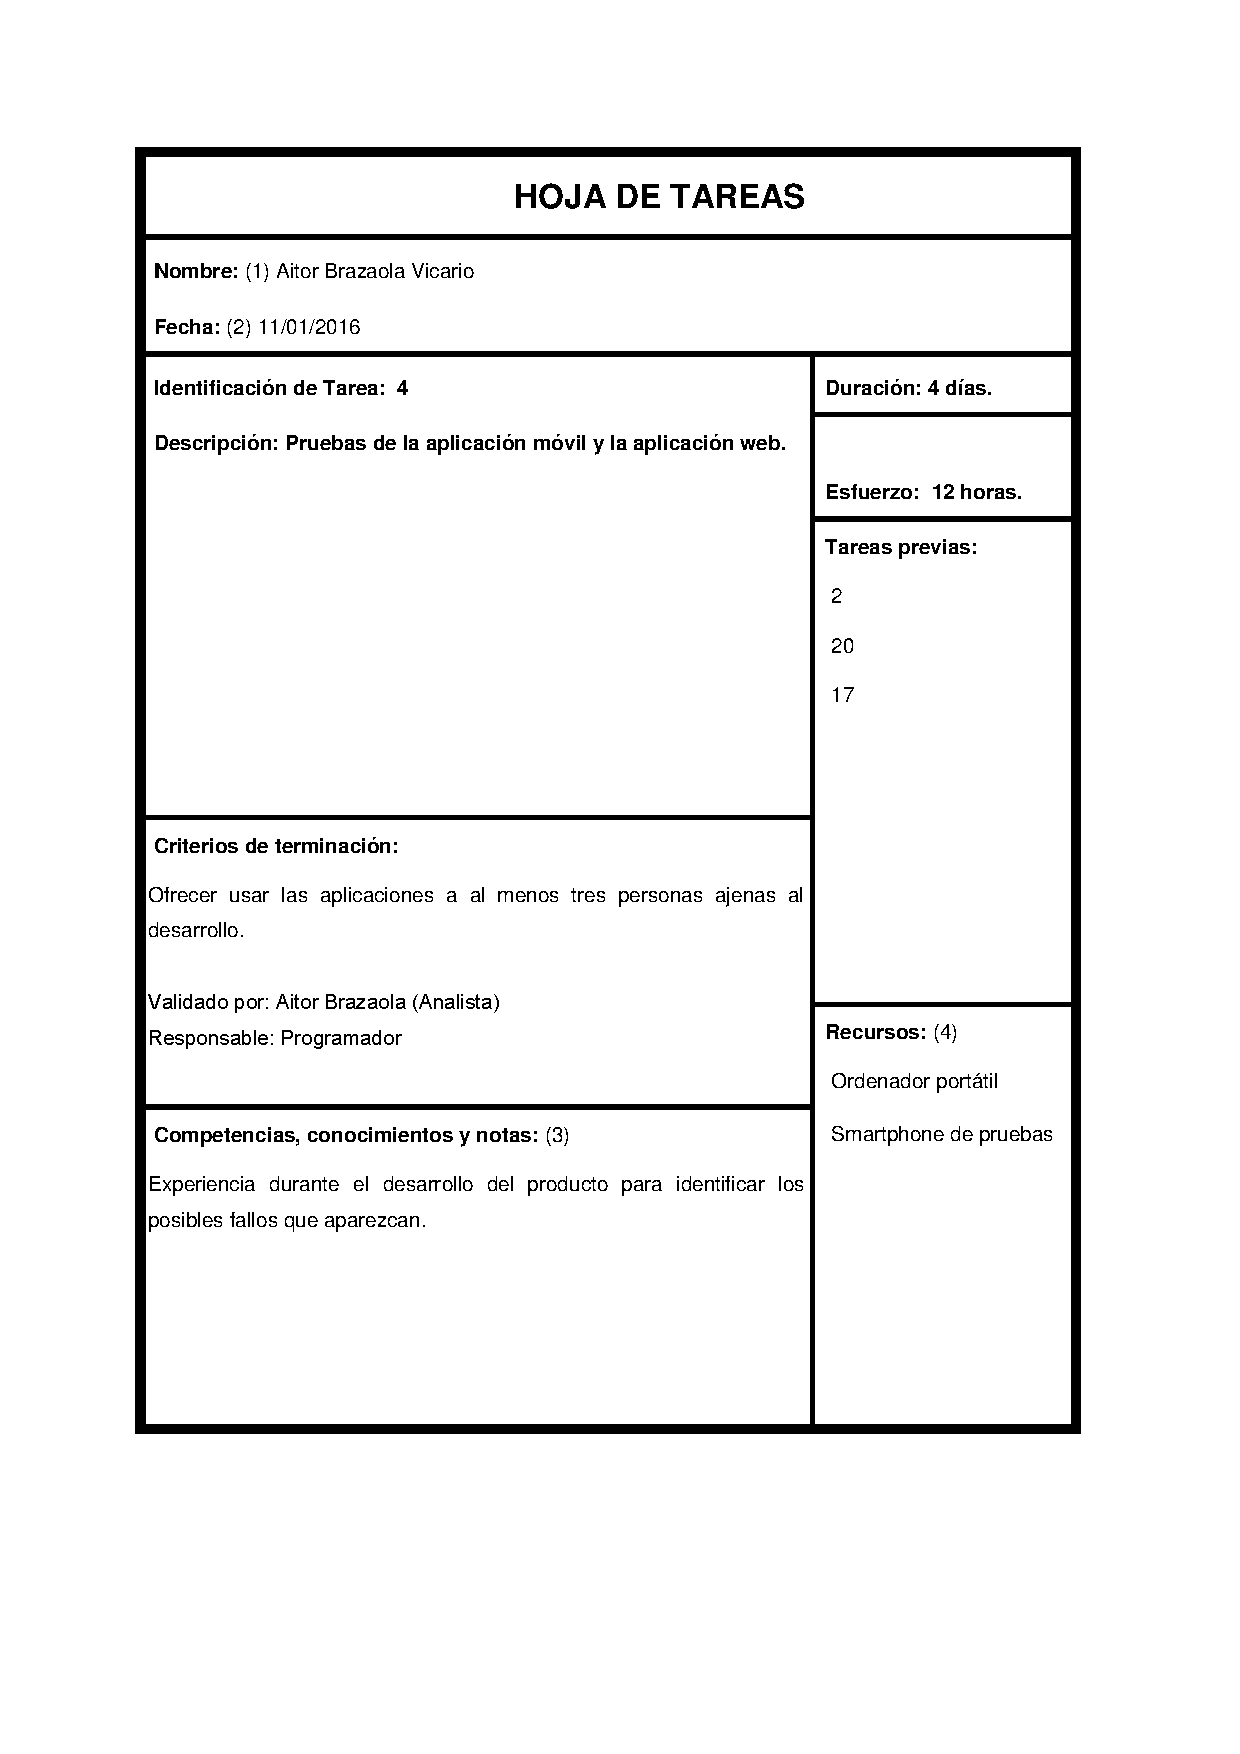
\includegraphics[width=0.9\textwidth]{fig/Tareas/4}
	\caption{Tarea 4.}
	\label{fig:t4}
\end{figure}

\chapter{Organización}
\section{Esquema organizativo}
La organización, como se piede ver en la imágen \ref{fig:esquemaorganizacion}, está compuesta en primer lugar por el Jefe de Proyecto, y el estudiante que hace los roles de programador y diseñador llevando a cabo el desarrollo del mismo.

\begin{figure}[h]
\centering
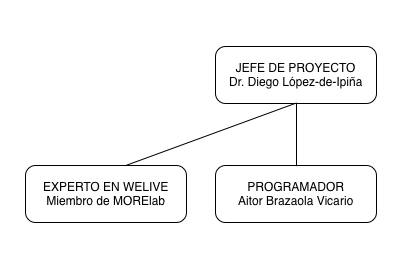
\includegraphics[width=0.7\linewidth]{fig/esquemaorganizacion}
\caption[Esquema de la organización]{Esquema de la organización}
\label{fig:esquemaorganizacion}
\end{figure}

Cada dos semanas se hará una sesión en la que se valorará el trabajo realizado y los cambios necesarios y si ya constituye suficiente producto como para considerar lo hecho una unidad funcional. 

\newpage
Los asistentes principales serán el programador principal y el jefe de proyecto y los detalles que se expongan se recogerán en el acta de la reunión, se puede ver la plantilla utilizada en la figura \ref{fig:Actareunion}, y se les dará prioridad frente al resto de funciones por implementar, evitando continuar el desarrollo por el camino equivocado.

\begin{figure}[h]
\centering
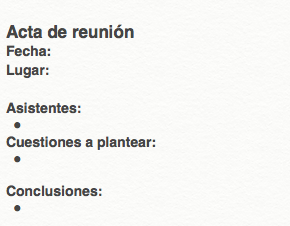
\includegraphics[width=0.7\linewidth]{fig/Actareunion}
\caption[Plantilla de acta de reunión]{Plantilla de acta de reunión}
\label{fig:Actareunion}
\end{figure}

\section{Plan de recursos humanos}
El estudiante al ser la única persona física que compone el equipo va a necesitar desarrollar diferentes roles durante todo el proyecto, si bien es cierto, que en momentos puntuales puede verse ayudado de otros compañeros del laboratorio en el que se encuentra, la mayor parte del proyecto es desarrollado por él. A continuación, se detallan los roles que desempeña en el proyecto:

\begin{description}
	\item[Programador:] Es el encargado de crear toda la lógica del programa, así como de realizar las diferentes configuraciones en los equipos responsables de que la plataforma funcione. Sus funciones cubren también las fases tempranas de diseño del software, creación del esquema de datos y llevar a cabo las pruebas correspondientes para detectar errores.
	\item[Diseñador:] Es el encargado de diseñar una interfaz de usuario que se adapte a todas las pantallas disponibles y que toda la aplicación sea accesible para personas con discapacidades así como asegurar una experiencia de usuario satisfactoria y una navegación coherente entre las diferentes secciones de la web.
\end{description}

Además del estudiante, el proyecto cuenta con su Jefe de Proyecto que es el encargado de aprobar todos los cambios y propuestas que el estudiante considere interesantes para mejorar el producto, estará presente en las reuniones y será el encargado de marcar las fechas de los hitos más importantes del proyecto.

\section{Estimación de cargas de trabajo}
\begin{itemize}
    \item 1. Definición de requisitos: 15 horas.
    \item 2. Aplicación web: 168 horas.
    \begin{itemize}
        \item 2.1. Creación de prototipo de la aplicación web: 15 horas.
        \item 2.2. Modelado de datos: 9 horas.
        \item 2.3. Diseño del software: 15 horas.
        \item 2.4. Implementación de las funciones básicas del portal: 45 horas.
        \item 2.5. Creación de un sistema de usuarios: 18 horas.
        \item 2.6. Implementación de los avisos por mail: 9 horas.
        \item 2.7. Securización de enlaces: 3 horas.
        \item 2.8. Mensajes de error: 3 horas.
        \item 2.9. Internacionalización: 6 horas.
        \item 2.10. Despliegue en servidor: 12 horas.
        \item 2.12. Autenticación con Google: 6 horas.
        \item 2.13. Autenticación con Facebook: 6 horas.
        \item 2.14. Integración con WeLive: 6 horas.
        \item 2.15. API Rest: 12 horas.
        \item 2.16. Corrección de errores visuales en pantallas de alta densidad: 3 horas.
    \end{itemize}
    \item 3. Aplicación móvil: 60 horas.
    \begin{itemize}
        \item 3.1. Prototipo de aplicación móvil: 3 horas.
        \item 3.2. Formación en la tecnología elegida para el desarrollo: 12 horas.
        \item 3.3. Implementación de la app móvil: 45 horas.
    \end{itemize}
    \item 4. Pruebas: 12 horas.
\end{itemize}


\chapter{Condiciones de ejecución}
El proyecto va a ser desarrollado en las oficinas que dispone Deustotech en el edificio de ingeniería de la Universidad de Deusto, el estudiante tiene acceso a un puesto con conexión a internet donde puede trabajar con su ordenador portátil. El calendario de trabajo vendrá definido por el que sigue Deustotech con las festividades correspondientes.

El horario que se ha propuesto inicialmente es de tres horas diarias, preferiblemente por las mañanas, empezando a las 10:00 y terminando la jornada a las 13:00, aunque en situaciones especiales pueda haber cambios en la franja horaria, se respetarán siempre las tres horas diarias.

El estudiante va a utilizar su propio ordenador portátil modelo Apple MacBook Pro para programar ya que es donde se encuentra mas confortable con las herramientas de desarrollo, Deustotech pone a disposición  los siguientes medios necesarios para el desempeño de la labor:
\begin{description}
	\item[Pantalla externa:] Utilizada para ampliar las capacidades del equipo portátil propio del estudiante.
	\item[Conexión a internet:] Para la búsqueda de información y recursos necesarios para el desarrollo del proyecto.
	\item[Mobiliario y cableado] Una sección de mesa y silla donde el estudiante puede situarse físicamente a trabajar y poder conectar su equipo.
\end{description}

\section{Interlocución}
Dado que por la propia naturaleza del proyecto no se puede tener contacto con un cliente final, toda comunicación acerca de decisiones de diseño y soporte serán directamente con el tutor del proyecto, pudiendo concertar una reunión en cualquier momento tras solicitarlo vía email o simplemente cuando esté disponible en la oficina que tiene situada en las instalaciones de Deustotech.

La relación con el tutor es directa y por tanto no se necesitan personas ni procedimientos intermedios, acortando los tiempos de gestión de cualquier tipo de comunicación, el tutor tomará decisiones desde el punto de vista del usuario final y sus recomendaciones serán muy tenidas en cuenta.

\section{Control de cambios}
Todos los cambios y peticiones recibidas durante el proceso de desarrollo del proyecto se gestionarán a través del siguiente procedimiento:
\begin{enumerate}
	\item Comunicación vía soporte electrónico de la modificación solicitada.
	\item Solicitud de reunión con el Jefe del proyecto para consultar su opinión y decidir si se implementa.
	\item En caso afirmativo, valorar lo cambios técnicos necesarios en la plataforma antes de implementar.
	\item En caso que los cambios sean técnicamente factibles y encajen en el presupuesto y el calendario, proceder a la implementación.
	\item Modificar el plan de trabajo y el presupuesto.
\end{enumerate}

\section{Recepción de productos}
Los documentos tales como diseños, manuales y especificaciones funcionales, deberán ser previamente presentados al jefe de proyecto en una reunión concertada, una vez se cuente con su aprobación se pueden llevar a la siguiente etapa en la que en la mayor parte de las veces será necesaria una implementación de lo descrito.

Cada vez que haya una unidad funcional de software primero tiene que ser desplegada en los servidores de desarrollo que Deustotech dispone y una vez se encuentre disponible concertar una reunión con el jefe del proyecto para que realice una evaluación del software y en caso de que haya cambios o errores que solicite, sean corregidos con la máxima prioridad antes de continuar con el resto de tareas.
\newpage

\chapter{Planificación}
\section{Diagrama de precedencia}
\begin{figure}[H]
	\centering
	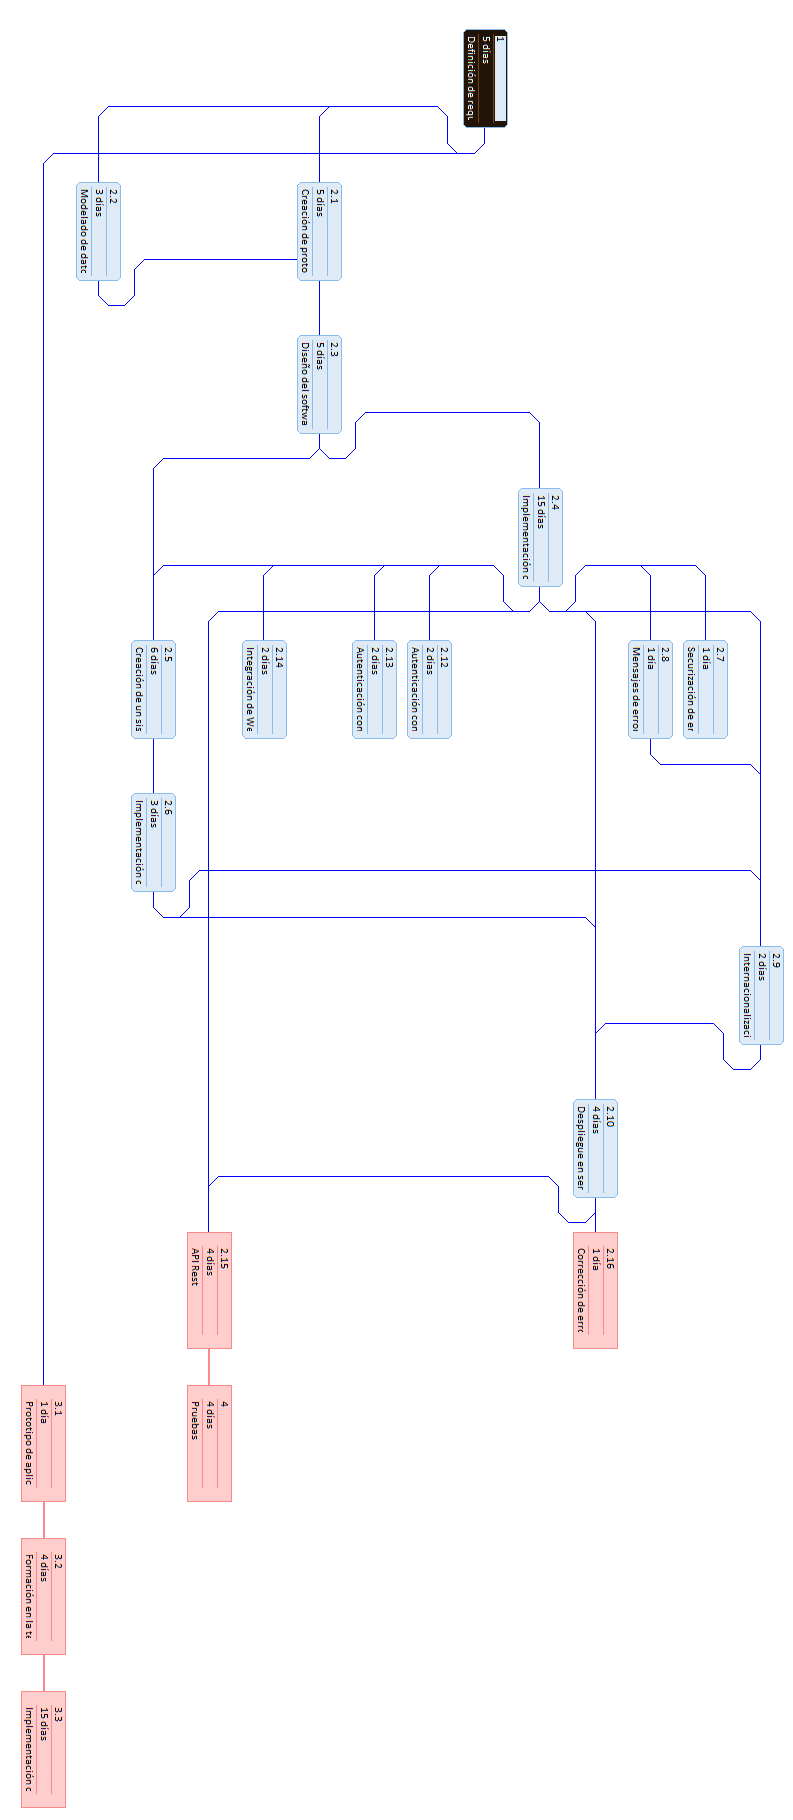
\includegraphics[width=210pt]{fig/precedencia}
	\caption{Diagrama de precedencia}\label{fig:precedencia}
\end{figure}

El desarrollo del proyecto se va a llevar a cabo durante la jornada de trabajo en DeustoTech MORELab de 4 horas diarias y solo se contará con una persona que desarrollará los siguientes roles:

\begin{description}
	\item[Programador:] Persona encargada de programar las estructuras de control de la plataforma.
	\item[Diseñador:] Persona encargada de el aspecto final con el que el usuario final va a interactuar.
	\item[Director de proyecto:] Persona a cargo de controlar el progreso del proyecto y de su organización.
	\item[Experto en plataforma WeLive:] Miembro del equipo de MORELab participante del desarrollo de la plataforma WeLive para asesorar técnicamente al equipo.
\end{description}

\newpage
\section{Diagrama de GANTT}
\begin{figure}[H]
    \centering
    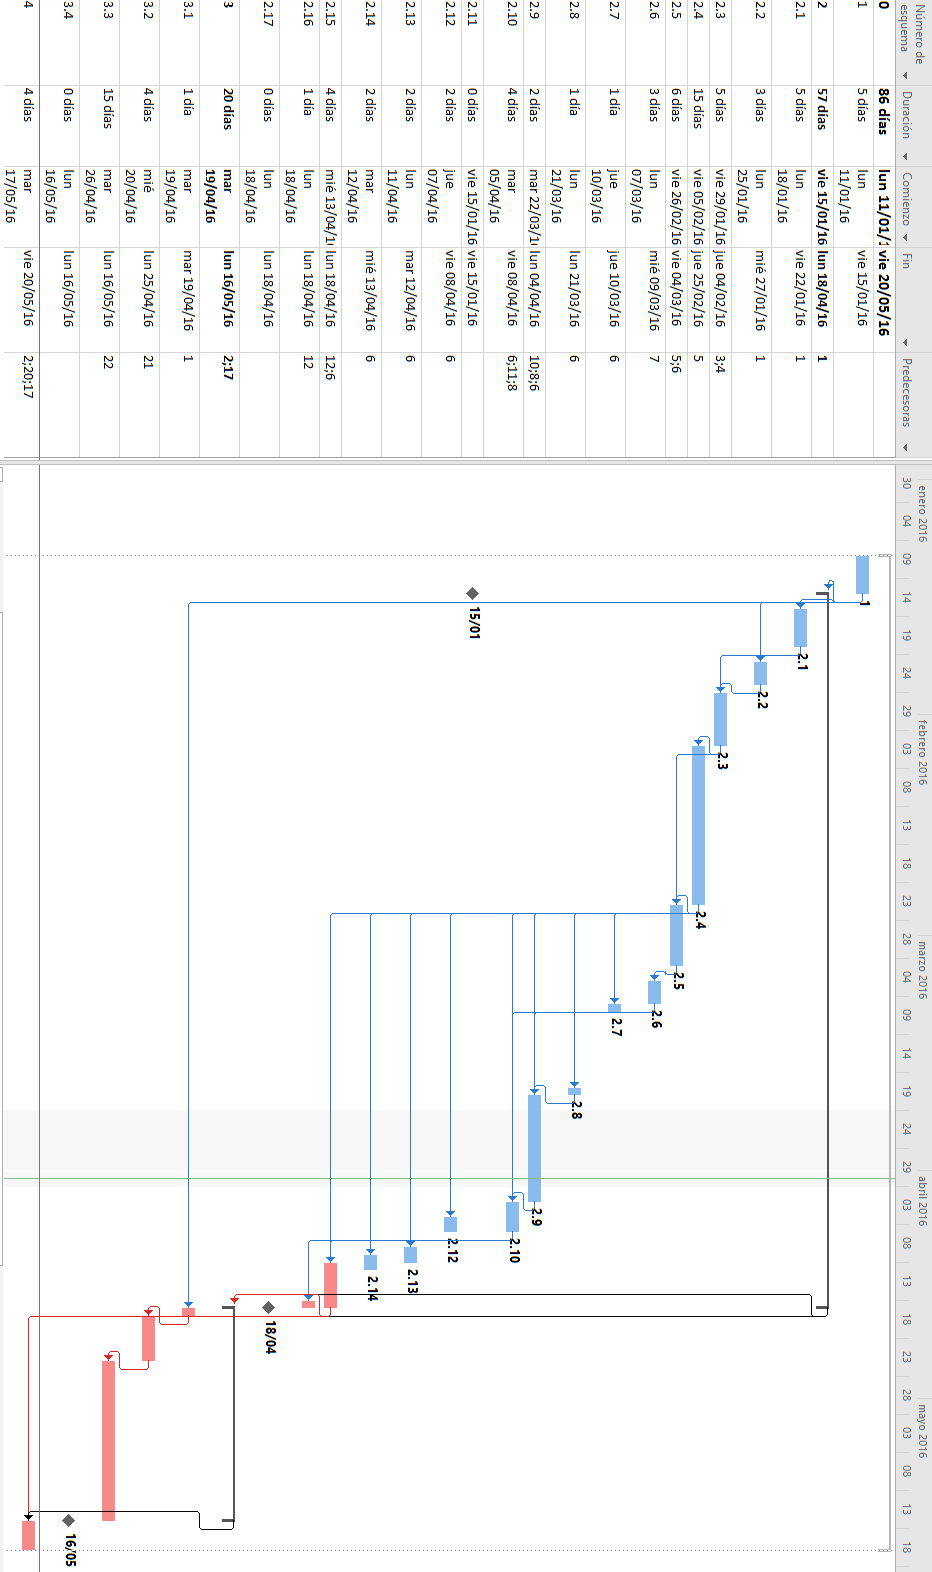
\includegraphics[width=340pt]{fig/gantt}
    \caption{Diagrama de GANTT}\label{fig:gantt}
\end{figure}

\section{Estimación de cargas de trabajo por perfil}
A continuación, se especifica la carga de trabajo estimada para cada perfil del proyecto sobre el total de 255 horas:
\begin{description}
   	\item[Programador:] 215 horas.
   	\item[Diseñador:] 22 horas.
   	\item[Director de proyecto:] 15 horas.
   	\item[Experto en plataforma WeLive:] 3 horas.
\end{description}   

\chapter{Presupuesto}
En el presupuesto se tendrá en cuenta únicamente las horas de trabajo ya que los equipos disponibles ya se tienen en propiedad por el programador y las instalaciones de DeustoTech, donde se realizará el proyecto.
\begin{table}[H]
   	\centering
   	\caption{Presupuesto por perfiles.}\label{tab:presupuestoperfiles}
   	\begin{tabular}{cccc}
   		\toprule
   		\textbf{Perfil} & \emph{Carga} & \emph{Precio} & \emph{Importe}\\
   		\midrule
   		Programador  & 255 h.     & 9€/h. & 2295€ \\
   		Diseñador   & 22 h.     & 9€/h. & 198€ \\
   		Director de proyecto & 12 h.     & 50€/h.  & 600€ \\
   		Experto en plataforma WeLive & 3 h.     & 6€/h. & 18€ \\
   		TOTAL & & & 3.111€\\
   		\bottomrule
   	\end{tabular}
\end{table}
     

\printbibliography[heading=bibintoc]

\appendix

\backmatter

\end{document}
